\documentclass[11pt,a4paper]{article}

\usepackage[utf8]{inputenc}
\usepackage[T1]{fontenc}
\usepackage[spanish,es-noquoting,es-nodecimaldot,es-tabla]{babel}
\usepackage{amsmath,amssymb}
\usepackage{siunitx}
\sisetup{detect-all, per-mode=symbol}
\usepackage{booktabs}
\usepackage{array}
\usepackage{graphicx}
\usepackage[section]{placeins}
\newcolumntype{L}[1]{>{\raggedright\arraybackslash}p{#1}}
\usepackage{microtype}
\setlength{\emergencystretch}{2em}
\usepackage[margin=2.5cm]{geometry}
\usepackage{xcolor}
\usepackage[colorlinks=true,linkcolor=azulosc,citecolor=azulosc,urlcolor=azulosc]{hyperref}

\definecolor{azulosc}{HTML}{1F4E79}
\definecolor{grisclaro}{HTML}{F2F2F2}

\usepackage{pgfplots}
\pgfplotsset{compat=1.16}
\usepackage{tcolorbox}
\tcbuselibrary{skins,breakable}
\newtcolorbox{nota}[1][]{colback=grisclaro, colframe=azulosc, boxrule=0.6pt,
  arc=2pt, left=6pt, right=6pt, top=5pt, bottom=5pt, breakable, #1}

\graphicspath{{figuras/}}

\title{Autogravedad contra mezcla de fases\\
       \large Una demo de ocho corridas PIC en la reducción de momento angular fijo}
\author{Notas de trabajo}
\date{25 de septiembre de 2026}

\begin{document}
\maketitle

\begin{abstract}
En la reducción de momento angular fijo con fondo isócrono, la teoría lineal
predice que la autogravedad de una componente de masa pequeña saca un modo de
la banda de frecuencias orbitales cuando el cociente $\eta$ entre el
corrimiento de frecuencias y el ancho de la banda pasa de $\eta_c\approx1.1$--$1.2$.
Esta demo pone a prueba esa predicción, y lo que la teoría lineal no alcanza,
con ocho corridas PIC de $10^4$ partículas sobre la Maxwelliana de Wilson, más
seis corridas de referencia sin perturbación. A amplitud baja la PIC reproduce
la teoría lineal: la frecuencia y la tasa de amortiguamiento del modo en la
banda al \SI{1}{\%}, la frecuencia de los modos discretos a $10^{-4}$ y la
respuesta persistente del borde abrupto. Cerca de la transición se aparta de
ella como anticipa el criterio de O'Neil, aun con $\varepsilon=0.075$: el
amortiguamiento se detiene y aparecen islas de partículas atrapadas junto al
borde de la banda. Y un modo discreto pegado al borde pierde amplitud a
$\varepsilon=0.1$, cosa que la teoría lineal no predice. Cada corrida tiene
figuras de espacio fase en $(r,p_r)$ y $(Q,J)$ y un video.
\end{abstract}

\begin{nota}
\textbf{Lo que muestra la demo, en cinco puntos.}
\begin{enumerate}
\item \textbf{La PIC reproduce la teoría lineal donde debe} (D1, D2, D3, D4, D8):
misma frecuencia y misma tasa de amortiguamiento del polo, al \SI{1}{\%}, hasta
que la señal cae a $10^{-2}$--$10^{-3}$ de su valor inicial.
\item \textbf{La transición existe en la simulación completa}: con $\eta<\eta_c$
la perturbación del potencial decae en unos pocos $\tau_1$ (D1, D2); con
$\eta>\eta_c$ oscila sin amortiguarse durante $20\,\tau_1$ (D3, D4).
\item \textbf{Cerca de la transición la dinámica es no lineal para amplitudes
chicas} (D5, D6): en $\eta=1$, con $\varepsilon=0.075$, la PIC sigue a la teoría
lineal durante $20\,\tau_1$ y después deja de decaer: en $30$--$44\,\tau_1$ el modo es
cuatro o cinco veces la predicción lineal, con la frecuencia algo corrida; con $\varepsilon=0.84$ el amortiguamiento se detiene a los
$5\,\tau_1$ y la amplitud vuelve a crecer. Es el régimen $\nu=\omega_b/\gamma\gtrsim1$.
\item \textbf{El atrapamiento se ve directamente}: en $(Q,J)$ las filas de acción
junto al borde se enrollan en una isla (D6, D7), y las partículas del borde
cambian su acción unas cien veces más que en la corrida sin perturbación.
\item \textbf{Un modo discreto pegado al borde no es robusto} (D3 contra D4): a
$\varepsilon=0.1$ el de $\eta=1.24$, a $2.5\times10^{-4}$ del borde, pierde un \SI{19}{\%}
de amplitud en $15\,\tau_1$, que la teoría lineal no amortigua; el de $\eta=2$,
separado, pierde un \SI{5}{\%} más que la predicción lineal. La diferencia está en
las partículas: el modo empuja a las del borde fuera del soporte, hasta su
resonancia, que en D3 está a $0.002$ en acción y en D4 a $0.026$.
\end{enumerate}
\end{nota}


\section{Los conceptos, en resumen}
\label{sec:conceptos}

Esta sección reúne lo indispensable para leer la demo. El desarrollo completo,
con las aproximaciones y las comprobaciones, está en el documento de la batería
$\eta$ (\texttt{docs/\allowbreak experimento\_\allowbreak eta/\allowbreak bateria\_\allowbreak eta.pdf}).

\subsection{El modelo}
\label{sec:modelo}

Una componente autogravitante de masa $a_0$ se mueve en un fondo fijo: el
isócrono de masa y escala unidad, $\Phi_{\rm iso}=-1/(1+\sqrt{1+r^2})$, con $G=1$.
Las masas se miden en unidades de la del fondo ($a_0=0.1$ es un décimo). Todas
las partículas tienen el mismo momento angular $L_0=2$:
\[
  f(r,p_r,L)=F(r,p_r,t)\,\delta(L-L_0),\qquad
  H=\tfrac12p_r^2+\Phi_{\rm iso}(r)+\Phi_{\rm self}(r,t)+\frac{L_0^2}{2r^2},
\]
con $\Phi_{\rm self}$ el potencial de la propia componente, que se recalcula por
Poisson en cada paso. El elemento de espacio fase es $8\pi^2L_0\,dr\,dp_r$. El
código es PIC: cada partícula es una capa esférica con un peso fijo; el
movimiento es unidimensional en $(r,p_r)$.

\paragraph{Ángulo y acción.} Cada órbita es una curva cerrada en $(r,p_r)$. Su
\emph{acción} $J=\frac1{2\pi}\oint p_r\,dr$ es el área encerrada sobre $2\pi$, y el
\emph{ángulo} $Q$ avanza uniformemente de $0$ a $2\pi$ en una vuelta radial. En un
potencial fijo $\dot J=0$ y $\dot Q=\Omega(J)$, la frecuencia radial. En el isócrono
solo, $\Omega(J)=(J+c)^{-3}$ con $c=\frac12(L_0+\sqrt{L_0^2+4})=2.414$: la frecuencia
\emph{decrece} con la acción, y la órbita circular ($J=0$) es la más rápida. Cerca
de ella, $r-r_c\approx\sqrt{2J/\kappa}\cos Q$ y $p_r\approx-\sqrt{2J\kappa}\sin Q$: $J$ es el
tamaño del epiciclo y $Q$ su fase. Con autogravedad el mapa $(r,p_r)\to(Q,J)$ se
calcula numéricamente en el potencial del equilibrio; en esta demo las
coordenadas $(Q,J)$ de las figuras son siempre las de ese mapa fijo.

\subsection{El equilibrio y el dato inicial}
\label{sec:equilibrio}

Cualquier $F$ que dependa solo de $J$ es estacionaria, pero $J$ se define en el
potencial total, que incluye el de la propia $F$: el equilibrio se construye
iterando hasta la autoconsistencia (\texttt{equilibrio.py}).

\paragraph{La distribución: la Maxwelliana de Wilson.} Se escribe en la energía,
\[
  F_{\rm eq}=A\,E_\gamma(g,x),\qquad x=\frac{E_t-E}{T}\ (E<E_t),\qquad
  E_\gamma(g,x)=\sum_{n\ge0}\frac{x^{g+n}}{\Gamma(g+n+1)} .
\]
Lejos del borde es una Maxwell--Boltzmann, $F\propto e^{-E/T}$; cerca de la energía de
corte $E_t$ se anula como $(E_t-E)^g$. $g=2$ es el modelo de Wilson y $g=1$ el de
King. El borde es la órbita de acción $J_t=0.138$ ($E_t=E(J_t)$), y la
temperatura $T=(E_t-E_c)/W_0$ con $W_0=3$. Es monótona en la energía: no tiene
modos radiales inestables (Antonov). Se eligió porque su borde de vacío es el
objeto de los teoremas de Hadžić y colaboradores (\S\ref{sec:borde}).

\paragraph{La perturbación.} El dato inicial es el equilibrio más una perturbación
en el ángulo,
\[
  F=F_{\rm eq}(J)\,\big[1+\varepsilon\,s(J)\cos Q\big],\qquad s=(J/J_t)^{3/2}.
\]
Tiene media cero en $Q$: no cambia la masa ni el equilibrio. El factor $s(J)$ la
hace lisa en la órbita circular ($J^{3/2}\cos Q\propto J\,(r-r_c)$). Físicamente,
$\cos Q$ agrupa las partículas en fase: la componente respira radialmente.

\paragraph{Las partículas.} Una por nodo de una malla regular en $(Q,J)$:
$N_{rc}=400$ acciones en $[0,J_t]$ por $N_{pc}=25$ ángulos, $N=10^4$. Su posición
$(r,p_r)$ sale de invertir el mapa del equilibrio; la perturbación está en los
\emph{pesos}, no en las posiciones. Es una partida silenciosa: no hay ruido de
muestreo.

\subsection{La banda de frecuencias y la mezcla de fases}
\label{sec:banda}

Las acciones del soporte, $[0,J_t]$, giran con frecuencias en la banda
$[\Omega_{\min},\Omega_{\max}]=[\Omega(J_t),\Omega(0)]$, de ancho $\Delta\Omega$. Sin
autogravedad cada punto de $(Q,J)$ avanza a su propio ritmo,
\[
  \delta F(Q,J,t)=\varepsilon F_{\rm eq}s\cos\big(Q-\Omega(J)t\big),
\]
y el patrón inicial se \emph{cizalla}: las franjas de $\cos Q$ se inclinan y se
afinan en $J$. Cualquier observable lineal, como el potencial $\delta\Phi$ o un
armónico $h_1$, es una suma de fasores $e^{-i\Omega(J)t}$ que se desfasan, y decae
(lema de Riemann--Lebesgue). Es la \emph{mezcla de fases}: no hay disipación, la
información se va a escalas cada vez más finas en $J$. El tiempo en que el
armónico $k=1$ se desfasa por completo es
\[
  \tau_1=\frac{2\pi}{\Delta\Omega}\qquad(\approx 280\text{--}560\ \text{en la demo}).
\]
La forma del decaimiento la fijan los bordes de la banda: un borde donde el peso
se anula como $|J-J_e|^\alpha$ da una cola $t^{-(\alpha+1)}$.

\subsection{La autogravedad: el modo colectivo}
\label{sec:modo}

Con autogravedad, $\delta F$ produce $\delta\Phi$ y $\delta\Phi$ empuja a las partículas.
La ecuación linealizada,
\[
  \partial_t\delta F+\Omega(J)\,\partial_Q\delta F-F_{\rm eq}'(J)\,\partial_Q\delta\Phi=0 ,
\]
admite soluciones colectivas $\propto e^{i(Q-\omega t)}$. Su frecuencia compleja
$\omega-i\gamma$ decide todo:
\begin{itemize}
\item si $\omega$ cae \emph{dentro} de la banda, hay partículas resonantes
($\Omega(J)=\omega$) que absorben energía del modo: se amortigua con tasa $\gamma>0$
(amortiguamiento de Landau);
\item si cae \emph{fuera}, no hay resonancia y el modo oscila sin amortiguarse:
un \emph{modo discreto}, $\gamma=0$.
\end{itemize}
La posición en la banda se mide con $x=(\omega-\Omega_{\min})/\Delta\Omega$: $0<x<1$
dentro, $x<0$ por debajo. La gravedad es atractiva y empuja el modo hacia
abajo, hacia $\Omega_{\min}$, el borde de las órbitas más amplias.

\subsection{El criterio $\eta$}
\label{sec:eta}

La intensidad del acoplamiento se mide por cuánto corre la autogravedad las
frecuencias orbitales, comparado con el ancho de la banda:
\[
  \eta=\frac{\delta\Omega}{\Delta\Omega/\bar\Omega},\qquad
  \delta\Omega=\frac{\bar\Omega-\bar\Omega_{\rm iso}}{\bar\Omega_{\rm iso}},
\]
con $\bar\Omega$ la frecuencia media pesada por la masa en el equilibrio
autoconsistente y $\bar\Omega_{\rm iso}$ la misma para las mismas órbitas en el
isócrono solo. Con $\eta\ll1$ la dispersión de frecuencias gana y todo se mezcla;
con $\eta\gtrsim1$ el acoplamiento puede sacar un modo de la banda. En la familia
de la demo, $\eta$ crece con la masa algo más despacio que linealmente
($\eta/a_0$ baja de $15$ a $12$ entre $a_0=0.0065$ y $0.17$): $\eta=1$ en $a_0=0.075$.

\paragraph{Lo que dice la teoría lineal.} \texttt{lineal.py} resuelve la ecuación
linealizada en una malla $(Q,J)$ sin partículas, y de la cola se extrae el polo
$\omega-i\gamma$ (tabla~\ref{tab:lineal}). Al crecer $\eta$ el modo baja hacia
$\Omega_{\min}$ y se amortigua cada vez menos, y entre $\eta=1$ y $1.24$ cruza el borde
y queda un modo discreto: $\eta_c\approx1.1$--$1.2$.

\begin{table}[!htbp]
\centering
\small
\begin{tabular}{lrrcrrL{3.9cm}}
\toprule
caso & $a_0$ & $\eta$ & banda $[\Omega_{\min},\Omega_{\max}]$ & $x$ & $\gamma/\Delta\Omega$ & régimen lineal\\
\midrule
A1 & 0.0065 & 0.10 & $[0.0610,\,0.0723]$ & $\sim0.5$ & $\sim0.5$ & amortiguamiento rápido\\
A3 & 0.042 & 0.59 & $[0.0655,\,0.0791]$ & 0.14 & 0.17 & amortiguado\\
A4 & 0.075 & 1.00 & $[0.0698,\,0.0857]$ & 0.03 & 0.023 & amortiguado, en el borde\\
L5 & 0.097 & 1.24 & $[0.0727,\,0.0902]$ & $-0.01$ & 0 & modo discreto pegado al borde\\
L6 & 0.170 & 2.00 & $[0.0828,\,0.1055]$ & $-0.19$ & 0 & modo discreto separado\\
\midrule
G1a & 0.0069 & 0.10 & $[0.0610,\,0.0723]$ & $\approx0$ & -- & borde abrupto ($g=1$): respuesta que persiste\\
\bottomrule
\end{tabular}
\caption{Los equilibrios de la demo y su polo lineal (del barrido de la batería
$\eta$). Todos son Wilson con $J_t=0.138$, $W_0=3$, $L_0=2$ y $g=2$, salvo G1a, con
$g=1$ (King).}
\label{tab:lineal}
\end{table}

\subsection{El borde de vacío}
\label{sec:borde}

Hadžić, Rein, Schrecker y Straub (ARMA 2025) prueban, para el problema
linealizado con una masa central, una dicotomía en el exponente del borde: si
$F\propto(E_t-E)^g$ con $g>1$ las perturbaciones se amortiguan; si $1/2<g\le1$, no.
En la teoría lineal de este modelo se ve lo mismo: con el mismo $\eta=1$, $g\le1$
ya tiene modo discreto y $g\ge2$ sigue amortiguado; y con $\eta=0.1$ el borde
abrupto deja una respuesta que oscila en $\Omega_{\min}$ y decae cada vez más
despacio, mientras que la del borde suave se apaga. Una lectura: la relación de
dispersión contiene $\int F_{\rm eq}'/(\Omega-\omega)\,dJ$, y con
$F_{\rm eq}'\propto(J_t-J)^{g-1}$ esa integral diverge en $\omega\to\Omega_{\min}$ si
$g\le1$: un acoplamiento arbitrariamente débil alcanza para ligar un estado en
el borde.

\subsection{Cuándo deja de valer la teoría lineal}
\label{sec:nolineal}

En un potencial fijo la ecuación de Vlasov es exactamente lineal en $F$, para
cualquier $\varepsilon$: la no linealidad entra solo por $\delta\Phi$. Cerca de una
resonancia $\Omega(J_r)=\omega$ una partícula siente un péndulo, con
\emph{frecuencia de rebote}
\[
  \omega_b=\sqrt{|\Omega'(J_r)|\,|\delta\Phi|}\;\propto\;\sqrt{\varepsilon}.
\]
La onda atrapa partículas en un tiempo $\sim2\pi/\omega_b$ y se amortigua en
$1/\gamma$. El cociente es el parámetro de O'Neil,
\[
  \nu=\omega_b/\gamma .
\]
Si $\nu\ll1$ la onda muere antes de atrapar y la teoría lineal vale para todo
$t$. Si $\nu\gtrsim1$ las partículas resonantes quedan atrapadas, el
amortiguamiento se detiene y la amplitud oscila y satura: el estado final no lo
da la teoría lineal. Al acercarse a la transición $\gamma\to0$, así que
$\nu\to\infty$ \emph{para cualquier amplitud}: en $\eta=1$, $\nu\approx11\sqrt\varepsilon$ y basta
$\varepsilon\approx0.008$ para $\nu=1$. \textbf{Lo que decide la linealidad no es
$\varepsilon$ sino $\nu$.} Es exactamente donde la PIC hace falta. Del lado discreto
($\eta>\eta_c$) no hay resonancia y la pregunta no lineal es otra: si el modo
sobrevive a amplitud finita, porque su frecuencia se corre con la amplitud y
uno pegado al borde puede entrar en la banda. El segundo parámetro,
$\mu=\omega_b/\Delta\Omega$, compara el atrapamiento con la mezcla de todo el
continuo; en la demo es siempre menor que $0.3$.

\section{La demo}
\label{sec:demo}

\subsection{Las corridas}

Ocho corridas cubren los regímenes de la sección~\ref{sec:conceptos}: los dos
lados de la transición a amplitud baja, el borde de la transición a amplitud
creciente, el modo discreto a amplitud grande y el borde abrupto
(tabla~\ref{tab:corridas}). Cada equilibrio tiene además una corrida de
referencia con $\varepsilon=0$ (las Z), que se resta para aislar la respuesta a la
perturbación. Son catorce simulaciones.

\begin{table}[!htbp]
\centering
\small
\setlength{\tabcolsep}{4pt}
\begin{tabular}{llrrrrrrrL{4.3cm}}
\toprule
corrida & equil. & $\eta$ & $g$ & $\varepsilon$ & $\nu$ & $\mu$ & $t_{\rm fin}$ & $t_{\rm fin}/\tau_1$ & qué muestra\\
\midrule
D1 & A1 & 0.10 & 2 & 1 & 0.17 & 0.09 & 11100 & 20 & acoplamiento débil: lineal aun con $\varepsilon=1$\\
D2 & A3 & 0.59 & 2 & 0.065 & 0.30 & 0.05 & 4600 & 10 & amortiguado, lineal\\
D3 & L5 & 1.24 & 2 & 0.1 & $\infty$ & 0.09 & 7200 & 20 & modo discreto junto al borde\\
D4 & L6 & 2.00 & 2 & 0.1 & $\infty$ & 0.10 & 5520 & 20 & modo discreto separado de la banda\\
D5 & A4 & 1.00 & 2 & 0.075 & 3.0 & 0.07 & 17200 & 44 & borde de la transición, no lineal\\
D6 & A4 & 1.00 & 2 & 0.84 & 10 & 0.23 & 5200 & 13 & borde de la transición, muy no lineal\\
D7 & L5 & 1.24 & 2 & 1 & $\infty$ & 0.27 & 7200 & 20 & el modo de D3 a amplitud grande\\
D8 & G1a & 0.10 & 1 & 1 & $\sim2$ & 0.11 & 11140 & 20 & borde abrupto (King)\\
\midrule
\multicolumn{10}{L{14.6cm}}{Referencias con $\varepsilon=0$: Z\_A1 (de D1), Z\_A3 (D2),
Z\_A4 (D5 y D6), Z\_L5 (D3 y D7), Z\_L6 (D4) y Z\_G1a (D8).}\\
\bottomrule
\end{tabular}
\caption{Las catorce corridas. $\nu=\omega_b/\gamma$ y $\mu=\omega_b/\Delta\Omega$, con
$\omega_b\propto\sqrt\varepsilon$ estimada de la solución lineal en $t=0$; $\nu=\infty$
indica un modo discreto ($\gamma=0$). En G1a el decaimiento tardío no es
exponencial y $\gamma$ está mal definido: el $\nu$ es solo indicativo. Cada
corrida de referencia dura lo mismo que la más larga de las que acompaña.}
\label{tab:corridas}
\end{table}

\paragraph{Por qué estas duraciones.} Las amortiguadas en régimen lineal duran
$10$--$20\,\tau_1$, lo suficiente para ver la cola después de la mezcla. En D5 y D6
la escala relevante es el periodo de rebote $2\pi/\omega_b$ ($5700$ y $1700$): las dos
cubren unos tres periodos de rebote, el tiempo en que la teoría de O'Neil
predice que el amortiguamiento se detiene y la amplitud oscila.

\begin{figure}[htbp]
\centering
\begin{tikzpicture}
\begin{axis}[width=0.78\textwidth, height=0.46\textwidth, xmin=0, xmax=2.2,
  ymode=log, ymin=0.08, ymax=200, xlabel={$\eta$}, ylabel={$\nu=\omega_b/\gamma$},
  ytick={0.1,1,10}, yticklabels={$0.1$,$1$,$10$},
  tick label style={font=\small}, label style={font=\small}]
  \fill[azulosc!6] (axis cs:0,0.08) rectangle (axis cs:2.2,1);
  \fill[orange!10] (axis cs:0,1) rectangle (axis cs:2.2,40);
  \fill[green!8] (axis cs:0,40) rectangle (axis cs:2.2,200);
  \fill[gray!25] (axis cs:1.1,0.08) rectangle (axis cs:1.2,200);
  \draw[gray, thin] (axis cs:0,40) -- (axis cs:2.2,40);
  \node[font=\footnotesize, azulosc, anchor=south east] at (axis cs:2.17,0.09) {lineal: la onda muere antes de atrapar};
  \node[font=\footnotesize, orange!60!black, anchor=north west] at (axis cs:0.03,38) {atrapamiento: la teoría lineal falla a tiempos largos};
  \node[font=\footnotesize, green!40!black, anchor=north west] at (axis cs:0.03,190) {modo discreto, $\gamma=0$};
  \node[font=\footnotesize, gray!70!black, rotate=90, anchor=south] at (axis cs:1.1,0.5) {$\eta_c$};
  \addplot[only marks, mark=*, mark size=2.4pt, azulosc] coordinates
    {(0.10,0.17) (0.59,0.30) (1.00,3.0) (1.00,10)};
  \addplot[only marks, mark=square*, mark size=2.2pt, red!70!black] coordinates {(0.13,2.4)};
  \addplot[only marks, mark=triangle*, mark size=3pt, green!40!black] coordinates
    {(1.24,70) (1.40,120) (2.00,80)};
  \node[font=\footnotesize, anchor=west] at (axis cs:0.13,0.17) {D1};
  \node[font=\footnotesize, anchor=west] at (axis cs:0.62,0.30) {D2};
  \node[font=\footnotesize, anchor=west] at (axis cs:1.03,3.0) {D5};
  \node[font=\footnotesize, anchor=west] at (axis cs:1.03,10) {D6};
  \node[font=\footnotesize, anchor=west] at (axis cs:0.16,2.4) {D8 ($g=1$)};
  \node[font=\footnotesize, anchor=north] at (axis cs:1.24,62) {D3};
  \node[font=\footnotesize, anchor=west] at (axis cs:1.43,120) {D7};
  \node[font=\footnotesize, anchor=west] at (axis cs:2.03,80) {D4};
\end{axis}
\end{tikzpicture}
\caption{Las corridas en el plano $(\eta,\nu)$. La franja gris es la transición
lineal, $\eta_c\approx1.1$--$1.2$. Arriba, fuera de escala, los modos discretos: ahí
no hay partículas resonantes y $\nu$ no aplica (D3 y D7 están en el mismo $\eta$,
separadas para que se lean). D8 está desplazada un poco en $\eta$ respecto de D1.}
\label{fig:mapa}
\end{figure}

\subsection{La configuración numérica}

Todas las corridas usan la misma: malla $r\in[0,20]$ con $\Delta r=0.1$,
$\Delta t=0.05$ (\texttt{courant}\,$=1$), integrador yoshida4, $N=400\times25=10^4$
partículas, autogravedad activa y una instantánea cada 200 pasos (10 unidades de
tiempo). Se corrieron una detrás de otra con 4 hilos OpenMP; los \texttt{.par}
están en \texttt{reproducir/corridas/12\_demo\_eta/} y todo el flujo en
\texttt{reproducir/scripts/demo\_eta.py} (apéndice~\ref{sec:reproducir}).

\subsection{Cómo se mide}
\label{sec:medida}

\paragraph{La perturbación del potencial.} En cada instantánea,
$\delta\Phi(r,t)=\Phi(r,t)-\Phi_{\rm iso}(r)-\Phi_{\rm self,eq}(r)$, en la malla del
código: no depende de ningún mapa, y es lo que los teoremas dicen que decae o no.
La parte debida a la perturbación se aísla restando la corrida Z del mismo
equilibrio y dividiendo por $\varepsilon$,
\[
  \delta\Phi_\varepsilon(r,t)=\frac{\delta\Phi(r,t;\varepsilon)-\delta\Phi(r,t;0)}{\varepsilon},
\]
que en régimen lineal no depende de $\varepsilon$. Su tamaño es $\|\delta\Phi\|$, el valor
rms en $3\le r\le15$, donde vive la componente.

\paragraph{El armónico $h_1$.} Con $(Q_j,J_j)$ del mapa del equilibrio,
$h_1=\sum_jf_jB(J_j)e^{-iQ_j}/\sum_jf_jB(J_j)$, con la función de prueba
$B=J^2e^{-(J-0.05)^2/0.05^2}$, y la misma resta de la corrida Z.

\paragraph{La referencia lineal.} \texttt{lineal.py} resuelve la ecuación
linealizada para el mismo equilibrio y el mismo dato inicial, sin partículas, y
da $\delta\Phi_{\rm lin}(r,t)$ y $h_{1,\rm lin}(t)$ con $\varepsilon=1$. La desviación no
lineal se mide como
\[
  \mathcal D(t)=\frac{\|\delta\Phi_\varepsilon-\delta\Phi_{\rm lin}\|}{\|\delta\Phi_{\rm lin}\|},
\]
y $t_{\rm nl}$ es el primer instante en que supera el \SI{10}{\%}.

\paragraph{Las figuras de espacio fase.} Cada partícula se dibuja en $(r,p_r)$ y en
$(Q,J)$, coloreada por su perturbación de peso, $f_j-f_{{\rm eq},j}=
\varepsilon F_{\rm eq}s\cos Q_0$: rojo donde la perturbación agrega masa y azul donde la
quita. Los pesos no cambian: el color es una etiqueta que viaja con la
partícula, y su patrón es la parte fina de $\delta F$. En las corridas Z el color es
$\cos Q_0$, una etiqueta sin efecto dinámico. En $(Q,J)$ cada fila de acción fija
avanza con su $\Omega(J)$, así que el patrón inicial de columnas se inclina: la
mezcla de fases se ve directamente como cizalla.

\section{Resultados}
\label{sec:resultados}

Los números de esta sección están en \texttt{exe/demo\_eta/resumen.txt}, que
escribe \texttt{demo\_eta.py figuras}. Las envolventes son el máximo de
$\|\delta\Phi\|$ en ventanas de $\pm50$ unidades de tiempo, algo más que una vuelta
radial; sin eso la oscilación del modo tapa la tendencia. El polo de la PIC se
ajusta como en la teoría lineal, con matrix pencil sobre $h_1$ en ventanas de
$\tau_1$.

\subsection{La transición a amplitud baja}
\label{sec:res_transicion}

\begin{figure}[htbp]
\centering
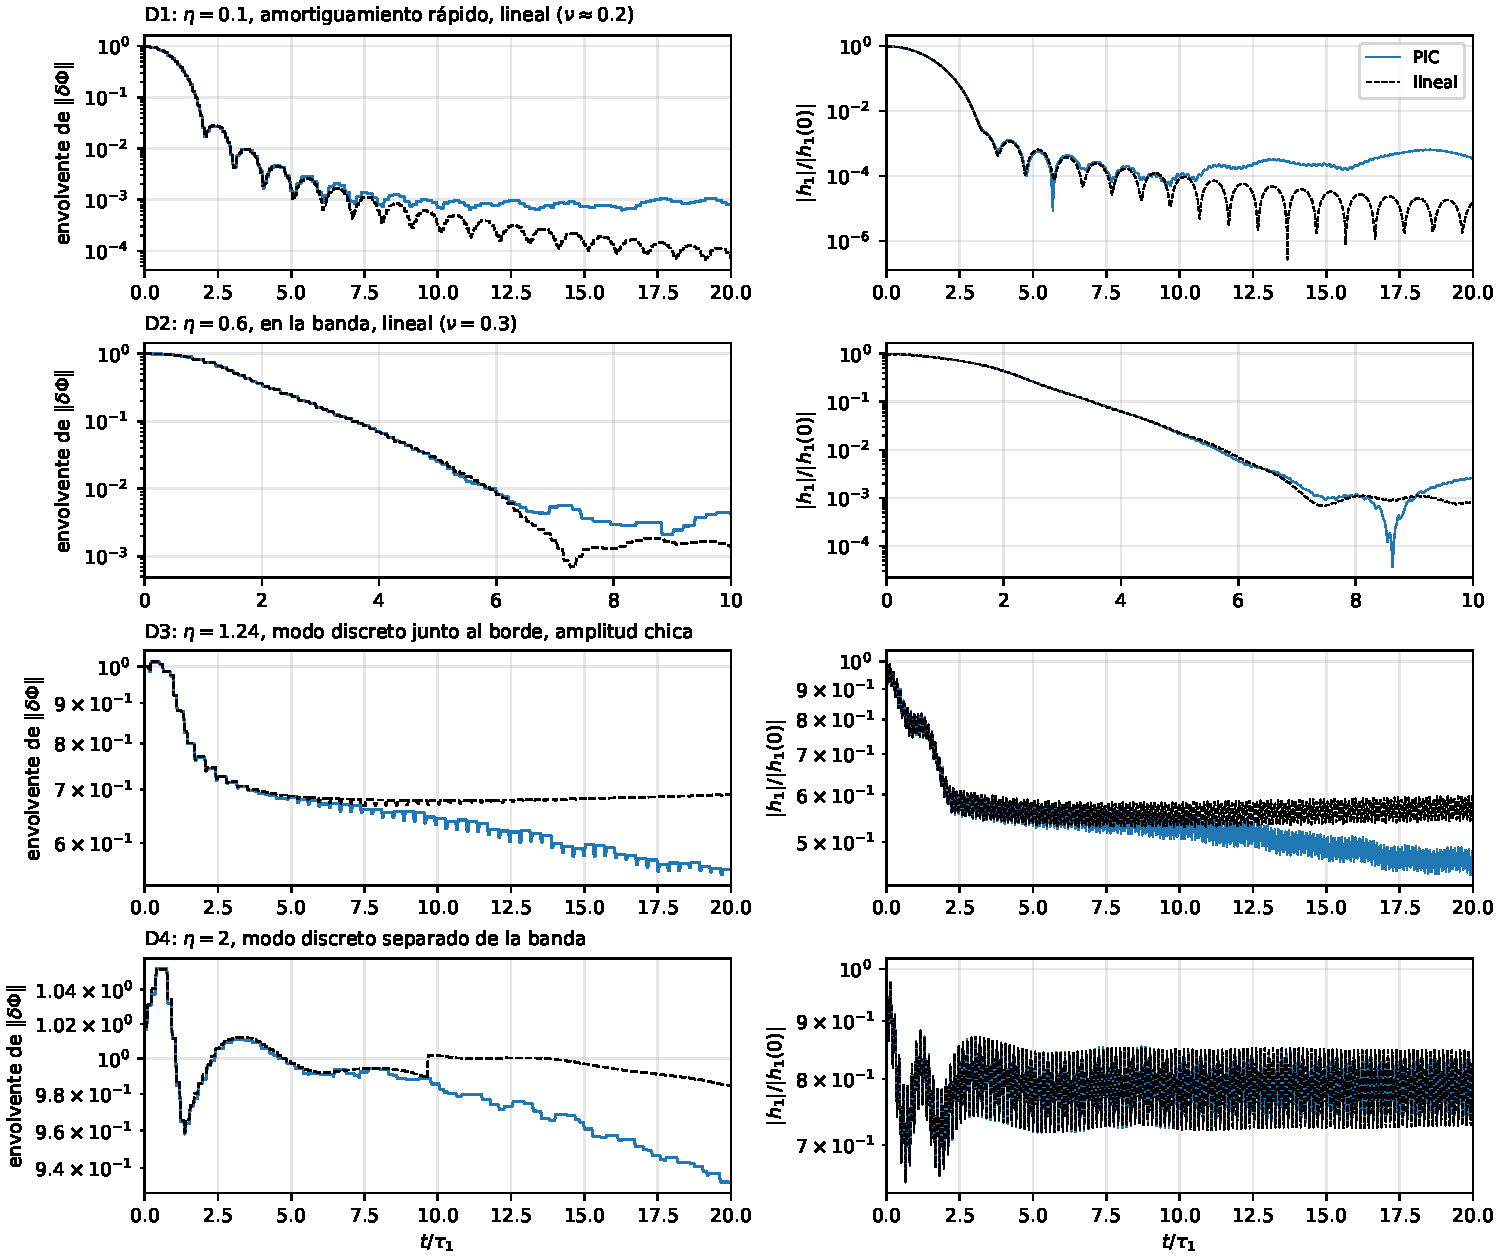
\includegraphics[width=\textwidth]{serie_transicion.pdf}
\caption{Las cuatro corridas en régimen lineal, a los dos lados de la
transición. Izquierda: envolvente de $\|\delta\Phi_\varepsilon\|$; derecha:
$|h_1|$, las dos relativas a su valor inicial. Azul, PIC; negro a trazos, teoría
lineal del mismo equilibrio y el mismo dato inicial. El tiempo está en unidades
de $\tau_1$ de cada equilibrio.}
\label{fig:transicion}
\end{figure}

\begin{table}[!htbp]
\centering
\small
\begin{tabular}{llcccccc}
\toprule
 & & \multicolumn{2}{c}{PIC} & \multicolumn{2}{c}{lineal} & & \\
\cmidrule(lr){3-4}\cmidrule(lr){5-6}
corrida & ventana & $\omega$ & $\gamma$ & $\omega$ & $\gamma$ & $R$ & $t_{\rm nl}/\tau_1$\\
\midrule
D1 ($\eta=0.1$) & $1$--$3\,\tau_1$ & 0.06568 & $2.59\times10^{-3}$ & 0.06568 & $2.57\times10^{-3}$ & 0.999 & 3.0\\
D2 ($\eta=0.6$) & $1$--$3\,\tau_1$ & 0.06796 & $1.27\times10^{-3}$ & 0.06796 & $1.28\times10^{-3}$ & 0.999 & 5.2\\
D3 ($\eta=1.24$) & $3$--$6\,\tau_1$ & 0.07242 & $4\times10^{-5}$ & 0.07244 & $<10^{-5}$ & 0.997 & 7.4\\
 & $10$--$20\,\tau_1$ & 0.07251 & $5\times10^{-5}$ & 0.07250 & $<10^{-5}$ & 0.933 & \\
D4 ($\eta=2$) & $3$--$6\,\tau_1$ & 0.07849 & $<10^{-5}$ & 0.07847 & $<10^{-5}$ & 0.999 & 9.6\\
 & $10$--$20\,\tau_1$ & 0.07847 & $<10^{-5}$ & 0.07848 & $<10^{-5}$ & 0.984 & \\
\bottomrule
\end{tabular}
\caption{El polo de $h_1$ en la PIC y en la teoría lineal. $R$ es el cociente de las
envolventes de $\|\delta\Phi\|$, PIC sobre lineal, en la misma ventana. $t_{\rm nl}$ es
el primer instante en que la envolvente del residuo PIC$-$lineal supera el
\SI{10}{\%} de la lineal; en D1 y D2 lo fija el piso de la medida
(\S\ref{sec:res_pisos}), no una desviación dinámica.}
\label{tab:polos}
\end{table}

\paragraph{Del lado amortiguado} (D1, D2) la PIC y la teoría lineal coinciden en la
frecuencia y la tasa del polo en tres o cuatro cifras (tabla~\ref{tab:polos}), y
las envolventes, al \SI{0.1}{\%} mientras la señal baja dos órdenes de magnitud.
D1 tiene $\varepsilon=1$: $\delta F/F_{\rm eq}$ es de orden uno y la evolución es lineal
igual, porque $\nu=0.17$. Es la ilustración directa de que $\varepsilon$ no es el
parámetro (\S\ref{sec:nolineal}). La PIC se separa de la teoría lineal solo
cuando la señal llega al piso de la medida: $6\times10^{-4}$ en D1, a los $3\,\tau_1$,
y $\sim2\times10^{-3}$ en D2, a los $5\,\tau_1$.

\paragraph{Del lado discreto} (D3, D4) la perturbación del potencial queda en un
\SIrange{55}{100}{\%} de su valor inicial durante $20\,\tau_1$, con la frecuencia
lineal a $10^{-4}$ relativo. La autogravedad sostiene una oscilación en la
simulación completa, no solo en la teoría lineal. Las dos corridas difieren en
cuánto dura:
\begin{itemize}
\item D4, con el modo bien separado de la banda ($x=-0.19$), pierde un
\SI{6.5}{\%} de envolvente entre $5$ y $20\,\tau_1$; la teoría lineal, un \SI{1.2}{\%}.
\item D3, con el modo a $2.5\times10^{-4}$ del borde ($x=-0.01$), pierde un
\SI{19}{\%} entre $5$ y $20\,\tau_1$ (de $0.685$ a $0.555$), mientras la teoría lineal
no pierde nada ($0.687$ y $0.690$). El
ajuste de $h_1$ da $\gamma\approx5\times10^{-5}$.
\end{itemize}
Lo que distingue a D3 se ve en las partículas del borde de la banda, las de
$J\approx J_t$. Un modo discreto no resuena con ninguna partícula del soporte, pero
su resonancia existe: está justo afuera, en la acción $J_r$ donde la frecuencia
orbital, prolongada más allá del borde, vale $\omega$,
\[
  J_r\approx J_t+\frac{\Omega_{\min}-\omega}{|\Omega'|},\qquad |\Omega'|\approx\frac{\Delta\Omega}{J_t}.
\]
En L5 el modo está a $2.5\times10^{-4}$ del borde y $J_r\approx J_t+0.002=0.140$; en L6, a
$4.3\times10^{-3}$, y $J_r\approx0.164$. Ahí no hay partículas en el equilibrio, pero la
amplitud finita del modo empuja a las del borde hacia afuera del soporte
(figura~\ref{fig:islas}): en D3 la acción máxima pasa de $0.138$ a $0.145$ en
$5\,\tau_1$ y a $0.151$ al final, más allá de $J_r$, y el cambio máximo de acción crece
sin saturar ($0.007$, $0.013$ y $0.020$ en $t=1800$, $3600$ y $7200$). En D4 la acción
máxima llega a $0.142$, lejos de su $J_r$, y el cambio de acción queda en
$0.003$--$0.004$; en las corridas sin perturbación, por debajo de $10^{-3}$. La
lectura es que \textbf{la amplitud finita puebla la resonancia de un modo discreto
pegado al borde}, y las partículas que llegan ahí le quitan energía; un modo
separado no la alcanza. En términos de escalas, la frecuencia de rebote de D3,
$\omega_b\approx1.5\times10^{-3}$, es seis veces la distancia al borde, y la de D4,
$2.3\times10^{-3}$, la mitad: para un modo discreto el cociente que decide la
linealidad sería $\omega_b/(\Omega_{\min}-\omega)$, no $\nu$. Es una interpretación
sostenida por las partículas; para confirmarla hay que ver que la pérdida de D3
desaparece al bajar $\varepsilon$ hasta que ese cociente sea menor que uno
($\varepsilon\approx0.003$), y que no cambia con $\Delta t$ ni con $N$
(\S\ref{sec:siguiente}).

\begin{figure}[htbp]
\centering
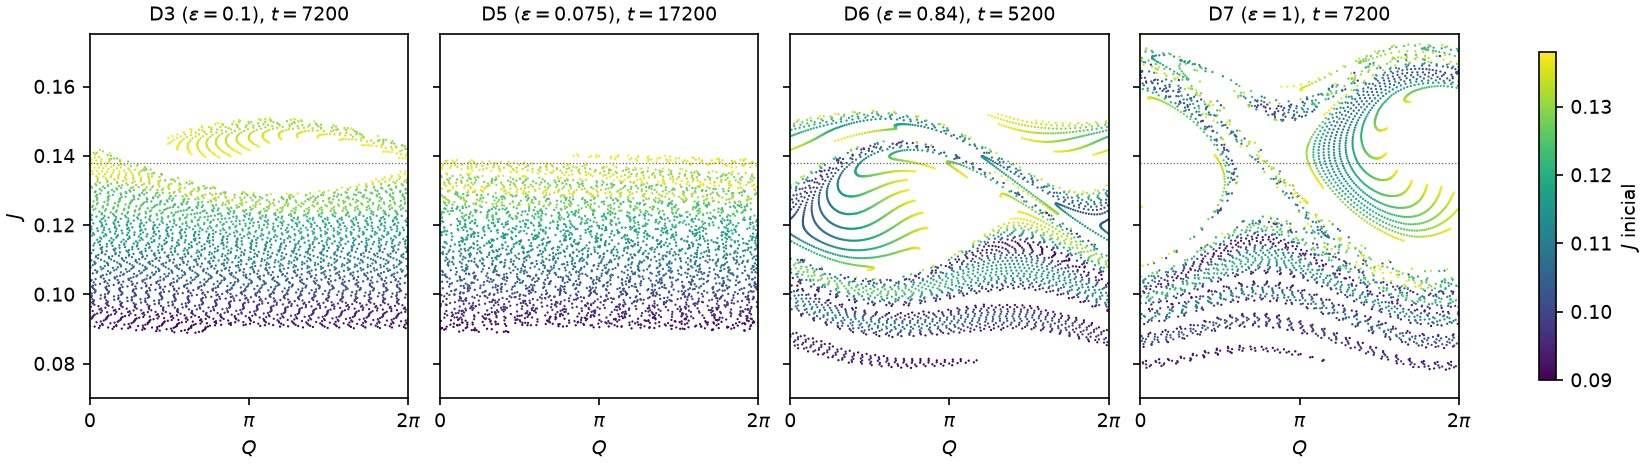
\includegraphics[width=\textwidth]{islas.jpg}
\caption{El borde de la banda al final de cuatro corridas: las partículas con
$J_0>0.09$ en $(Q,J)$, coloreadas por su acción \emph{inicial}. En la mezcla libre
cada color quedaría en su fila horizontal; la línea punteada es el borde del
soporte, $J_t$. D3: las filas del borde se despegan y forman un arco fuera del
soporte, hasta $J=0.151$. D5: el cambio es chico ($J\le0.140$). D6 y D7: islas de
partículas atrapadas, con su punto X y curvas cerradas alrededor del centro,
que se extienden hasta $J=0.153$ y $0.179$. La posición de la isla en $Q$ gira con la
onda y no tiene significado.}
\label{fig:islas}
\end{figure}

\subsection{El borde abrupto}
\label{sec:res_borde}

\begin{figure}[htbp]
\centering
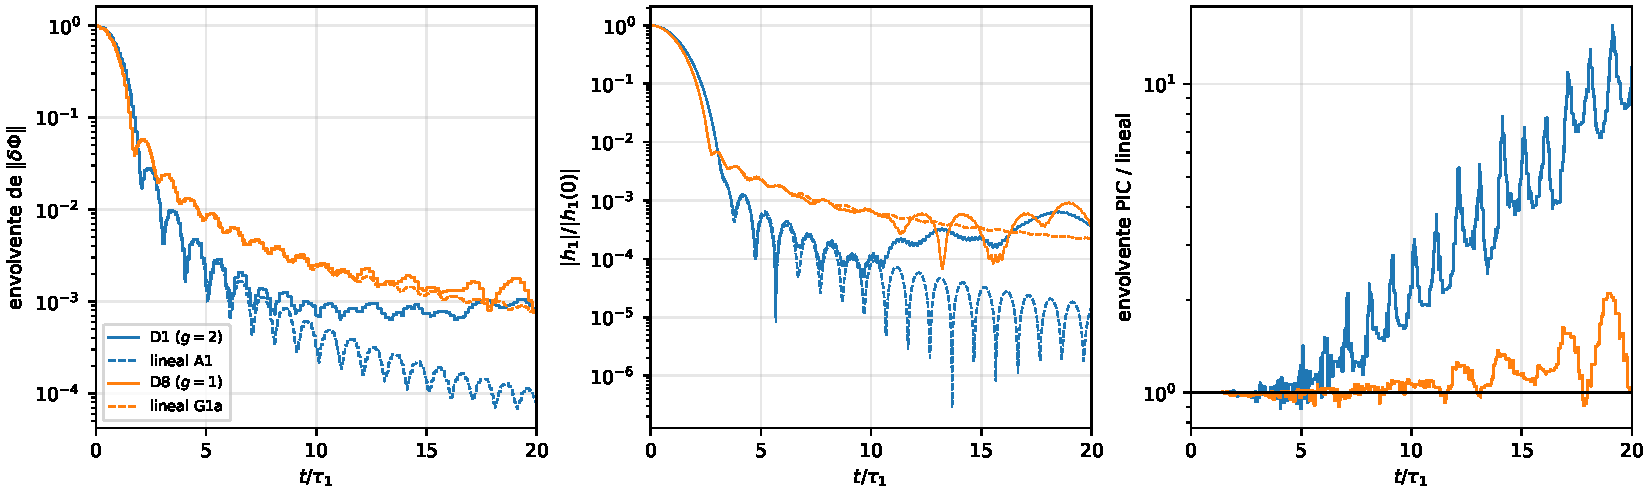
\includegraphics[width=\textwidth]{serie_borde.pdf}
\caption{El mismo $\eta=0.1$ con borde suave (D1, $g=2$) y abrupto (D8, $g=1$).
Izquierda y centro: envolvente de $\|\delta\Phi\|$ y $|h_1|$; en trazos, la teoría
lineal de cada equilibrio. Derecha: cociente de envolventes PIC/lineal. D1 llega
al piso de la medida hacia $5\,\tau_1$ (\S\ref{sec:res_pisos}); D8 queda por encima
hasta $\sim15\,\tau_1$.}
\label{fig:borde}
\end{figure}

D1 y D8 tienen la misma masa relativa ($\eta=0.1$) y difieren solo en el exponente
del borde de vacío (figura~\ref{fig:borde}). Hasta $2\,\tau_1$ son casi iguales;
después, la de borde abrupto decae mucho más despacio: en $10$--$20\,\tau_1$ su
envolvente es $2.6\times10^{-3}$, cinco veces la lineal de D1. La PIC sigue a la
teoría lineal de D8 al \SI{6}{\%} hasta $\sim15\,\tau_1$, y el polo tardío coincide:
$\omega=0.06088$ contra $0.06086$ en $10$--$20\,\tau_1$, justo debajo del borde de la
banda ($\Omega_{\min}=0.06101$). Es la respuesta de borde que en teoría lineal persiste
con $g\le1$ (la dicotomía de Hadžić), ahora en la simulación completa. Más allá de
$15\,\tau_1$ la señal de D8 llega al piso de las corridas con $\varepsilon=1$ y la PIC ya
no distingue los dos bordes.

\subsection{La no linealidad en el borde de la transición}
\label{sec:res_nolineal}

\begin{figure}[htbp]
\centering
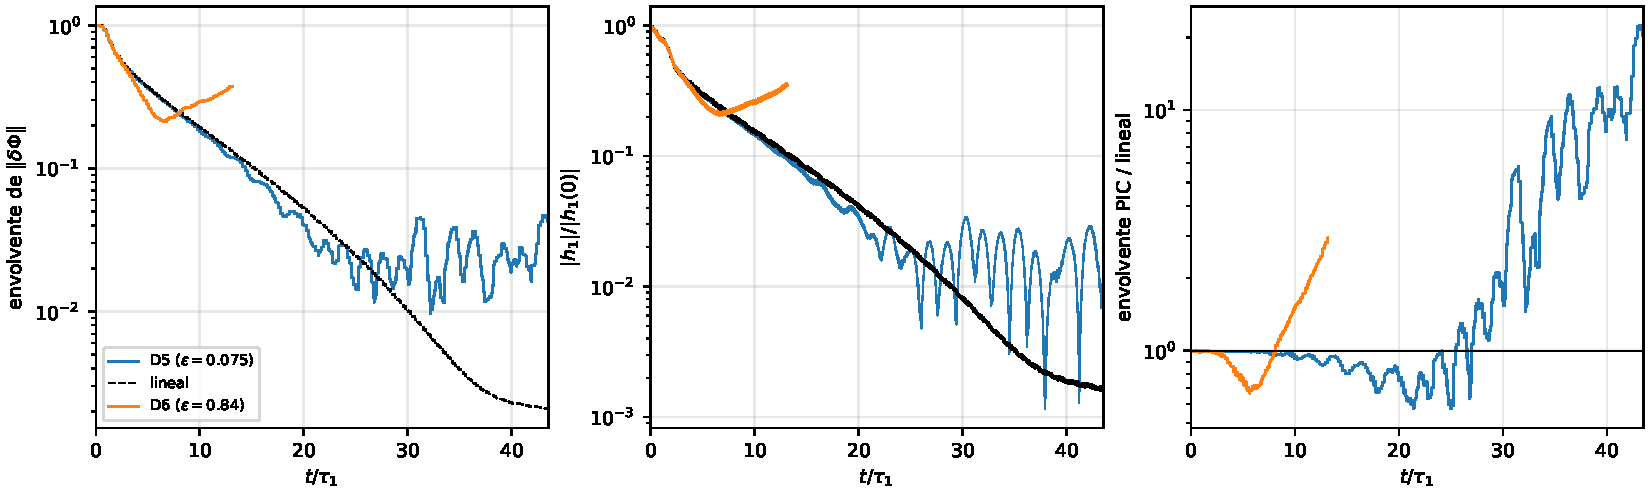
\includegraphics[width=\textwidth]{serie_nolineal.pdf}
\caption{El mismo equilibrio, A4 ($\eta=1$), a dos amplitudes: D5
($\varepsilon=0.075$, $\nu=3$) y D6 ($\varepsilon=0.84$, $\nu=10$). En trazos, la teoría
lineal, que es la misma para las dos una vez dividida por $\varepsilon$. Derecha:
cociente de envolventes PIC/lineal.}
\label{fig:nolineal}
\end{figure}

A4 está en el borde de la transición: el polo lineal está dentro de la banda
pero muy cerca de su borde ($x=0.03$) y se amortigua despacio,
$\gamma=3.7\times10^{-4}$. Con $\varepsilon=0.075$, $\delta F/F_{\rm eq}$ no pasa de \SI{7.5}{\%}
y cualquier criterio basado en $\varepsilon$ diría que el problema es lineal. El de
O'Neil dice lo contrario: $\nu=3$. La figura~\ref{fig:nolineal} muestra lo que pasa.

\paragraph{D5} ($\varepsilon=0.075$) sigue a la teoría lineal durante mucho tiempo: el
polo de $h_1$ coincide hasta $20\,\tau_1$ ($\gamma=3.8\times10^{-4}$ contra $3.7\times10^{-4}$) y
el cociente de envolventes baja lentamente de 1 a 0.9. Entre $20$ y $30\,\tau_1$ la
amplitud oscila alrededor de la curva lineal ($R=0.76$), y desde $\sim25\,\tau_1$ deja
de decaer: se queda en $1$--$4\times10^{-2}$ mientras la lineal baja a $2\times10^{-3}$. En
$30$--$44\,\tau_1$ la envolvente cruda es $4.7$ veces la lineal, y al final, veinte
veces, pero esa cifra mezcla dos cosas. Separando $\delta\Phi_\varepsilon(r)$ en su parte lisa
(suavizada sobre $0.5$ en $r$) y su parte fina:
\begin{itemize}
\item la parte lisa, proyectada sobre el perfil radial del modo lineal, es $4.5$
veces la lineal en $30$--$44\,\tau_1$ y oscila coherentemente a $\omega=0.0707$, contra
$0.0703$ de la lineal: un corrimiento hacia arriba como el de D6. $h_1$, que no pasa
por la malla, da un factor $\sim3$. Esto es el modo, y es lo que se afirma;
\item la parte fina, con escala de dos o tres celdas de la malla, es
$2\times10^{-2}$ al final, cincuenta veces la de la solución lineal, y crece con el
tiempo ($8\times10^{-3}$ en $20$--$30\,\tau_1$). Puede ser ruido de discretización
amplificado por $1/\varepsilon$ o estructura fina real de las partículas atrapadas; esta
demo no lo decide (\S\ref{sec:res_pisos}).
\end{itemize}
El tiempo de rebote inicial es $2\pi/\omega_b\approx5700\approx14\,\tau_1$: el
amortiguamiento se detiene a un par de periodos de rebote, como en el cuadro
de O'Neil. Las partículas junto al borde ($J\approx0.13$) cambian su acción en
$0.005$--$0.006$, y ese cambio se satura, como corresponde a partículas atrapadas
que oscilan en una isla en lugar de seguir absorbiendo energía.

\paragraph{D6} ($\varepsilon=0.84$) se aparta de la teoría lineal a los $3\,\tau_1$. Primero
decae más rápido que ella ($R=0.81$ en $5$--$10\,\tau_1$), después el amortiguamiento
se detiene ($\gamma=-4\times10^{-5}$ en $5$--$9\,\tau_1$, contra $+3.4\times10^{-4}$ lineal) y la amplitud vuelve a crecer: al final es el doble de la lineal. La frecuencia sube
un \SI{0.6}{\%} ($0.0709$ contra $0.0704$). El tiempo de rebote,
$2\pi/\omega_b\approx1700\approx4\,\tau_1$, es justo cuando el amortiguamiento se detiene. En
$(Q,J)$ la isla es visible (figuras~\ref{fig:islas} y~\ref{fig:fase_D6}): al final las
filas con $J\gtrsim0.11$ se enrollan en un ojo de gato, con su punto X, y las
partículas cambian su acción hasta en $0.048$, un tercio del soporte.

\subsection{El modo discreto a amplitud grande}
\label{sec:res_discreto}

\begin{figure}[htbp]
\centering
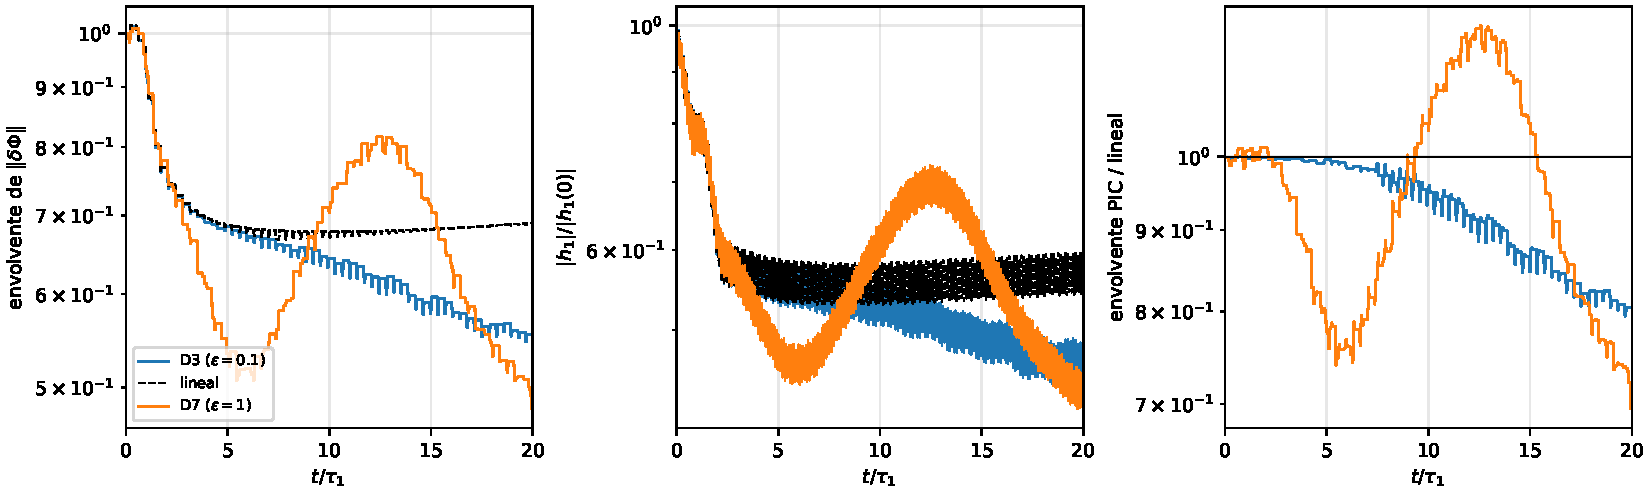
\includegraphics[width=\textwidth]{serie_discreto.pdf}
\caption{El modo discreto de L5 ($\eta=1.24$) a dos amplitudes: D3
($\varepsilon=0.1$) y D7 ($\varepsilon=1$).}
\label{fig:discreto}
\end{figure}

D7 lleva el modo de D3 a $\varepsilon=1$ (figura~\ref{fig:discreto}). El modo no se
amortigua: la envolvente oscila entre $0.5$ y $0.8$ de su valor inicial durante
las $20\,\tau_1$, con un periodo de $\sim14\,\tau_1$, en lugar de quedarse en $0.69$ como
la lineal. La frecuencia sube un \SI{0.4}{\%}, de $0.0725$ a $0.0728$, y queda justo
en el borde de la banda ($\Omega_{\min}=0.0727$): a amplitud grande el modo ya no está
separado del continuo. Las partículas cambian su acción hasta en $0.073$, más de
la mitad del soporte, y llegan hasta $J=0.179$, muy afuera de él: la banda
efectiva se extiende hacia abajo y el modo queda dentro de ella, pero atrapando
partículas en lugar de amortiguarse. La figura~\ref{fig:islas} muestra la isla
con su punto X. D3 y D7 juntas dicen que el modo sobrevive a amplitud finita,
pero no como un modo lineal: a amplitud chica pierde energía lentamente, y a
amplitud grande se reorganiza en una estructura no lineal que oscila.

\subsection{Qué limita la medida}
\label{sec:res_pisos}

Tres cosas fijan hasta dónde se puede seguir una señal que decae.
\begin{itemize}
\item \textbf{La discretización.} Al comienzo, PIC y teoría lineal difieren en
$\sim10^{-3}$ del valor inicial de $\|\delta\Phi\|$ en todas las corridas: es el
error combinado de las dos discretizaciones.
\item \textbf{La parte estática de segundo orden.} El residuo PIC$-$lineal tiene
una parte que no oscila, constante desde $\sim3\,\tau_1$: $5.7\times10^{-4}$ del valor
inicial en D1 y $7\times10^{-4}$ en D8. Es física: después de dividir por $\varepsilon$ crece
como $\varepsilon$ (entre D6 y D5 el cociente es 8--11 según la ventana, y el de las
amplitudes, 11.2), así que es un efecto $\propto\varepsilon^2$, el cambio del perfil radial promedio ($k=0$) que deja la
perturbación al mezclarse. Como no oscila, se puede restar; lo que queda es
$\sim2\times10^{-4}$.
\item \textbf{El ruido de la resta.} La corrida Z no es exactamente estacionaria:
su $\delta\Phi$ tiene una parte estática, el error de discretización del equilibrio,
y fluctuaciones. La resta las cancela casi del todo, pero lo que queda se divide
por $\varepsilon$: con $\varepsilon\approx0.07$ el piso es $\sim2\times10^{-3}$ (D2).
\item \textbf{La estructura fina.} La parte de $\delta\Phi_\varepsilon(r)$ con escala de pocas
celdas de la malla, que en la solución lineal es una fracción fija de la señal,
en la PIC tiene un piso: $4\times10^{-4}$ en D1 y D8 ($\varepsilon=1$), $4\times10^{-3}$ en D2
($\varepsilon=0.065$), de nuevo $\propto1/\varepsilon$. En D5 crece con el tiempo, hasta
$2\times10^{-2}$ a los $44\,\tau_1$. Para las colas largas conviene medir sobre la parte
lisa, o sobre $h_1$, que no pasa por la malla.
\end{itemize}
Como el segundo crece con $\varepsilon$ y el tercero decrece, hay una amplitud óptima
para seguir colas largas, del orden de $\varepsilon\approx0.3$--$0.5$, con un piso de unos
$5\times10^{-4}$. Es una estimación de estas corridas, no una medida.

\section{El espacio fase de cada corrida}
\label{sec:fase}

Cada figura muestra las $10^4$ partículas en cuatro instantes: el dato inicial,
$\tau_1/2$ (la cizalla empieza), $2\tau_1$ (la mezcla del armónico $k=1$ ya se completó
dos veces) y el final. Arriba en $(r,p_r)$, abajo en las variables ángulo-acción
del equilibrio. El color es la perturbación de peso de cada partícula
(\S\ref{sec:medida}): rojo, masa agregada; azul, masa quitada. Como el color viaja
con la partícula, lo que se ve es cómo el flujo transporta la perturbación.

\paragraph{Cómo leerlas.} En $t=0$ la perturbación $\cos Q$ ocupa las columnas de
la malla en $(Q,J)$ y, en $(r,p_r)$, una media luna roja del lado de $p_r<0$ y otra
azul enfrente: la componente respira. Con el tiempo cada fila de $J$ avanza con
su $\Omega(J)$: en $(Q,J)$ las columnas se inclinan y se afinan, y en $(r,p_r)$ la
media luna se enrolla en una espiral cada vez más apretada. Esa es la mezcla de
fases. Al final el patrón es más fino que la resolución de la figura y parece
ruido, pero no lo es: es la misma perturbación, enrollada. Lo que no es mezcla
es que las filas de $J$ \emph{dejen de ser horizontales} o que aparezcan
partículas por encima de la línea punteada, el borde $J_t$ del soporte: eso es
cambio de acción, y solo lo produce el campo propio. Es lo que distingue a D3, D6
y D7.

\begin{figure}[p]
\centering
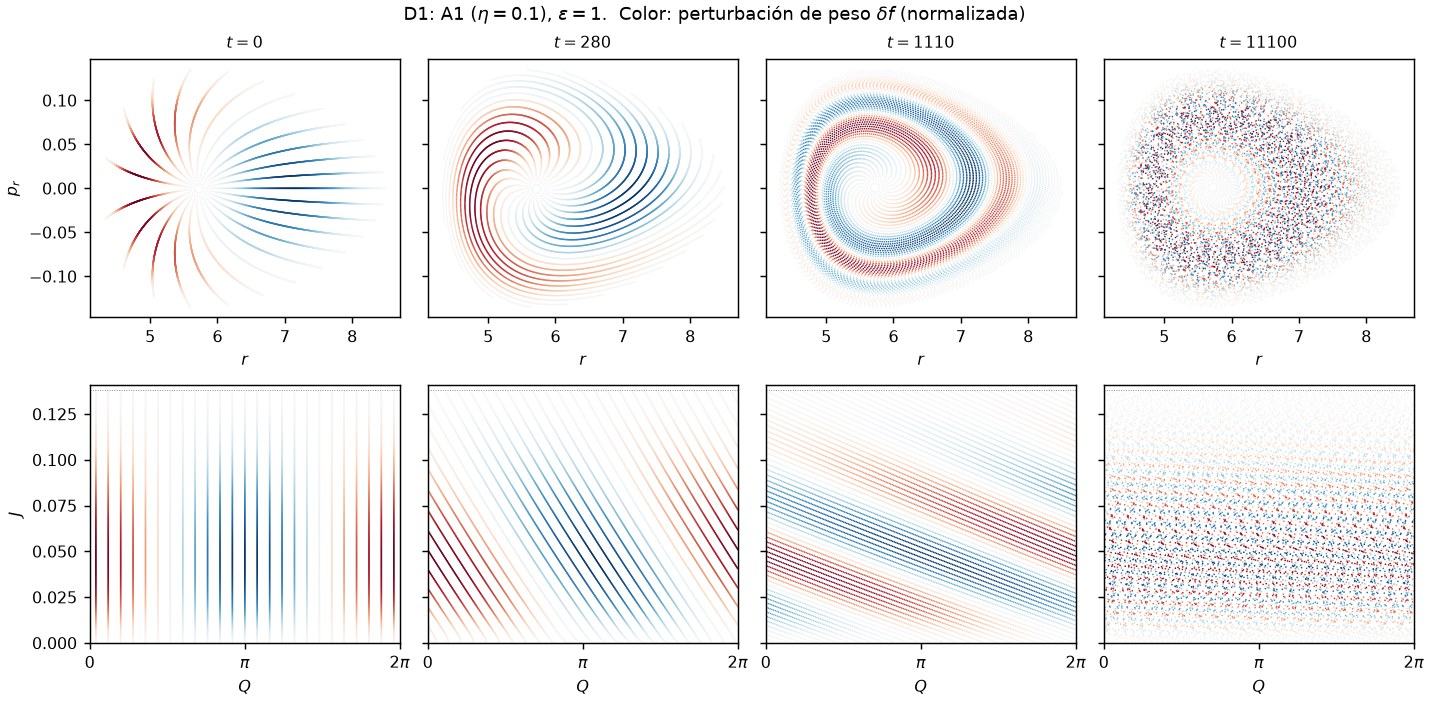
\includegraphics[width=\textwidth]{fase_D1.jpg}
\caption{D1: $\eta=0.1$, $\varepsilon=1$. La mezcla libre casi pura: las filas de $J$
siguen horizontales; el cambio máximo de acción es $0.002$.}
\label{fig:fase_D1}
\vspace{1.5em}
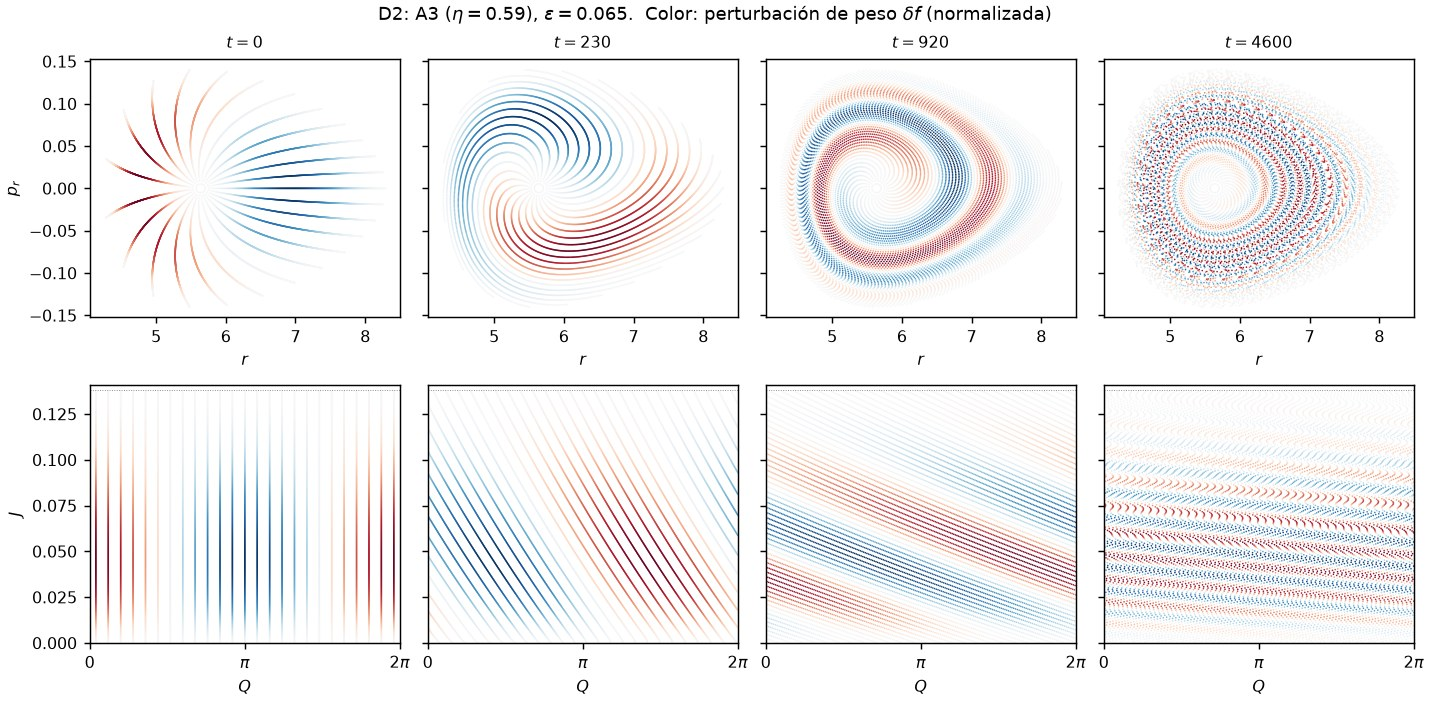
\includegraphics[width=\textwidth]{fase_D2.jpg}
\caption{D2: $\eta=0.59$, $\varepsilon=0.065$. Igual que D1 con una perturbación
quince veces menor; el modo colectivo se amortigua más despacio, pero en $(Q,J)$ no
se nota: la amplitud es chica.}
\label{fig:fase_D2}
\end{figure}

\begin{figure}[p]
\centering
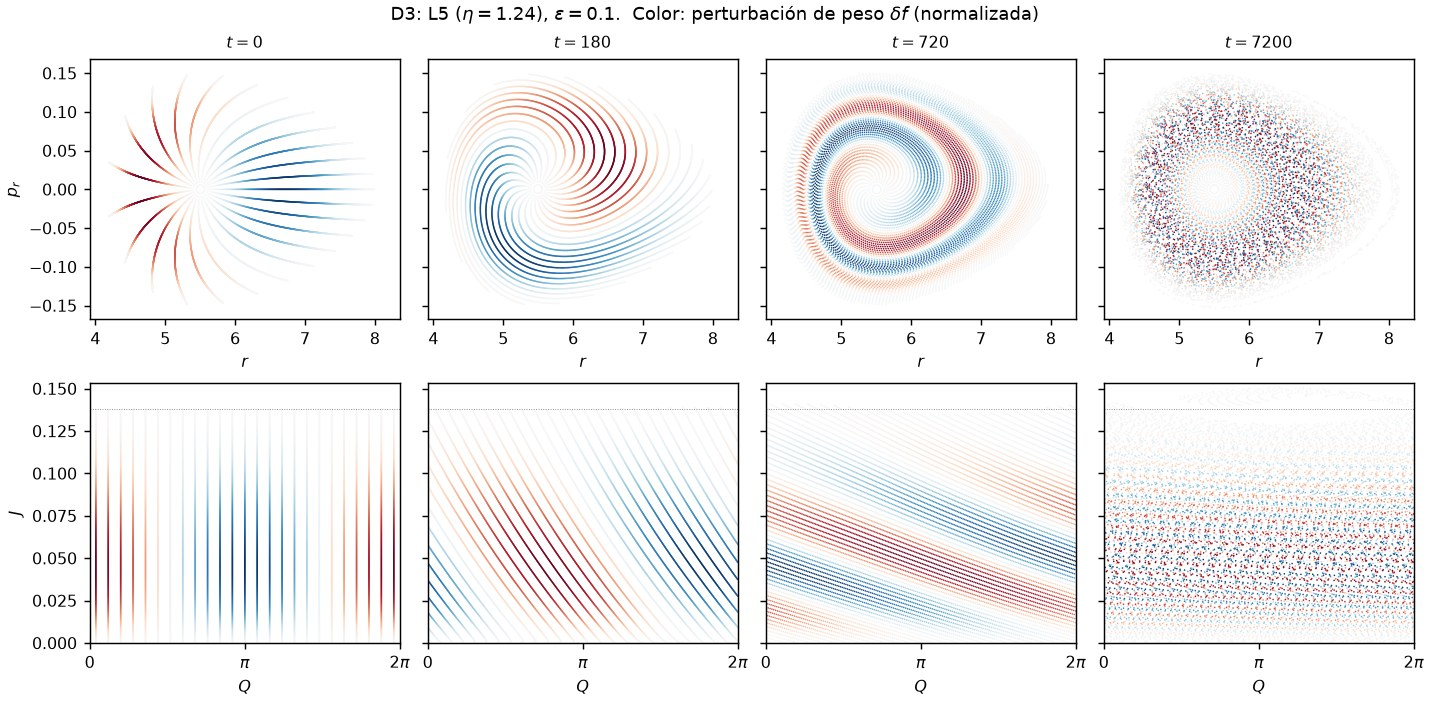
\includegraphics[width=\textwidth]{fase_D3.jpg}
\caption{D3: $\eta=1.24$, $\varepsilon=0.1$, modo discreto pegado al borde. En
$(Q,J)$ las filas del borde ($J\approx0.13$) se despegan hacia afuera del soporte;
su acción cambia hasta en $0.02$ al final (ampliación en la
figura~\ref{fig:islas}).}
\label{fig:fase_D3}
\vspace{1.5em}
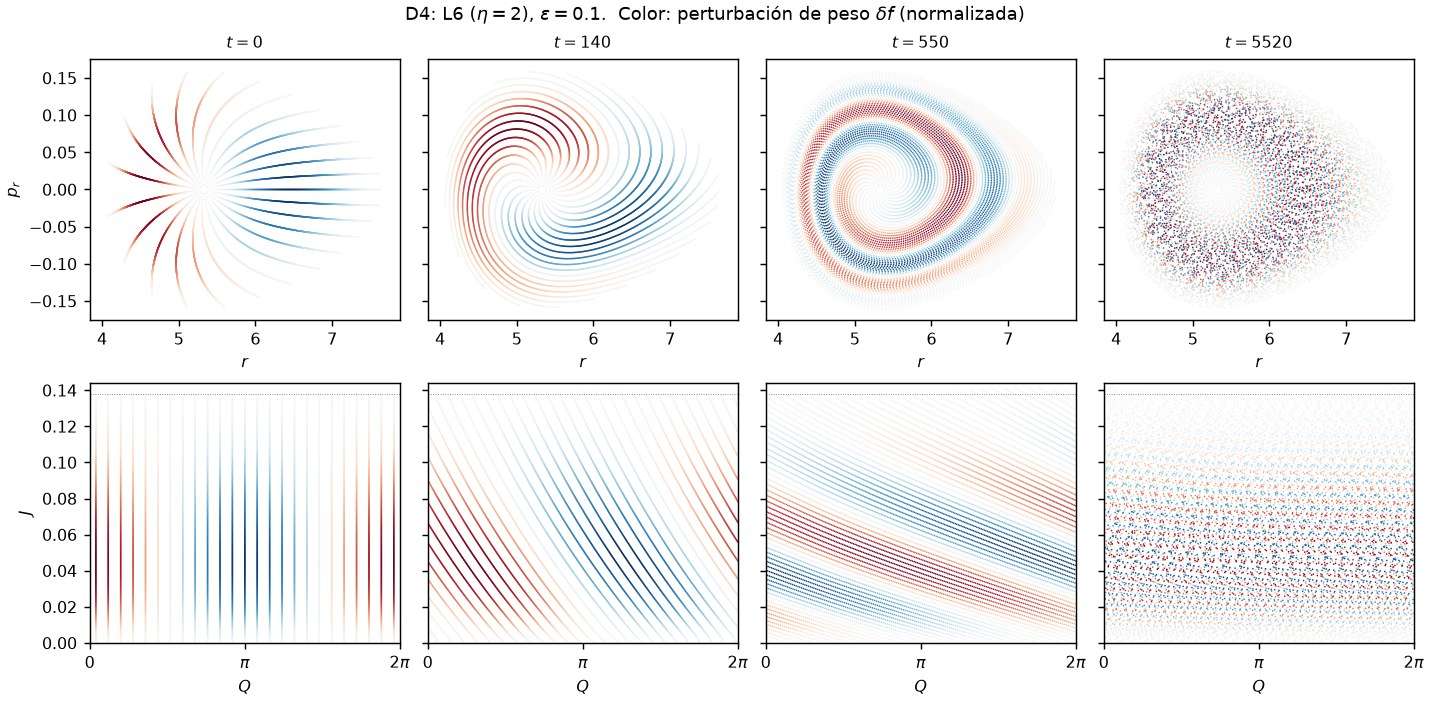
\includegraphics[width=\textwidth]{fase_D4.jpg}
\caption{D4: $\eta=2$, $\varepsilon=0.1$, modo discreto separado de la banda. Las
filas quedan horizontales (cambio máximo de acción $0.004$).}
\label{fig:fase_D4}
\end{figure}

\begin{figure}[p]
\centering
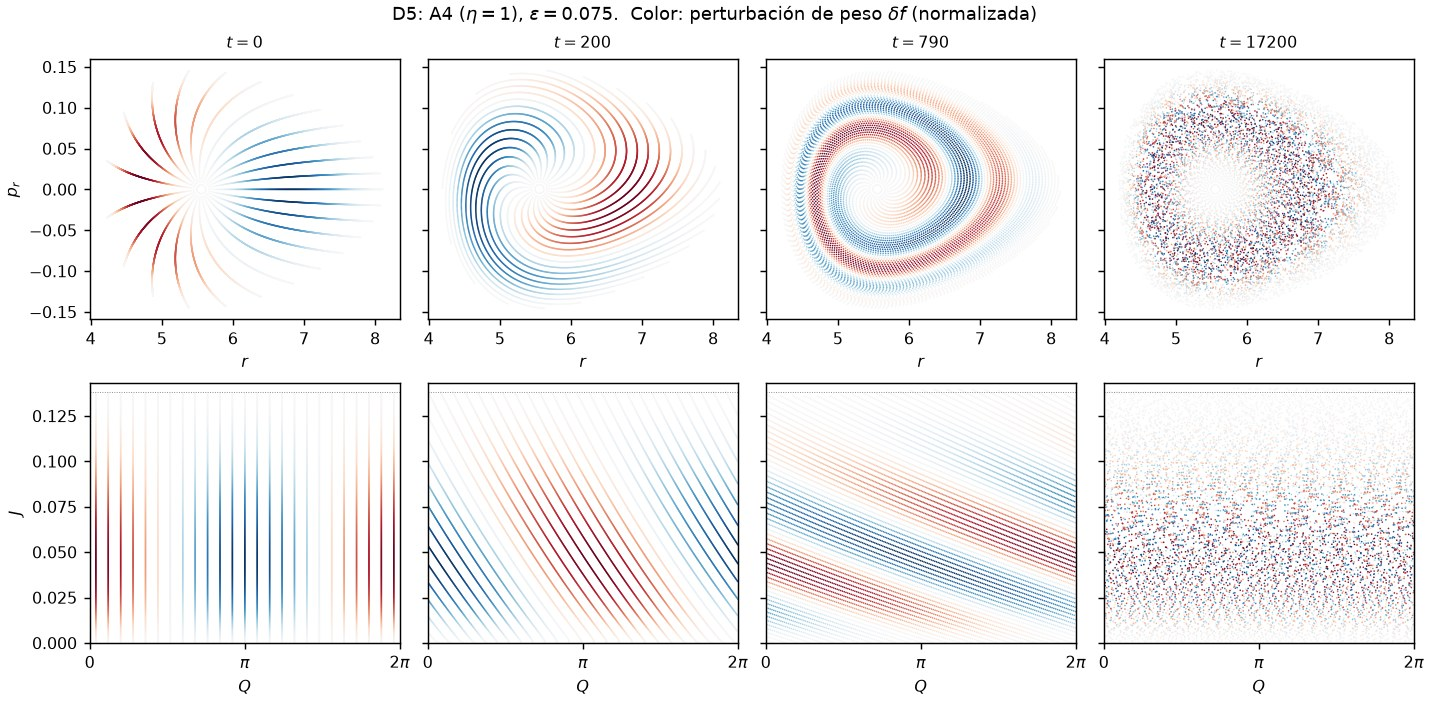
\includegraphics[width=\textwidth]{fase_D5.jpg}
\caption{D5: $\eta=1$, $\varepsilon=0.075$, hasta $t=17200$ ($43\,\tau_1$). El cambio de acción
se concentra junto al borde y se satura en $0.006$: demasiado chico para verse a
esta escala, pero unas quince veces el de la corrida sin perturbación.}
\label{fig:fase_D5}
\vspace{1.5em}
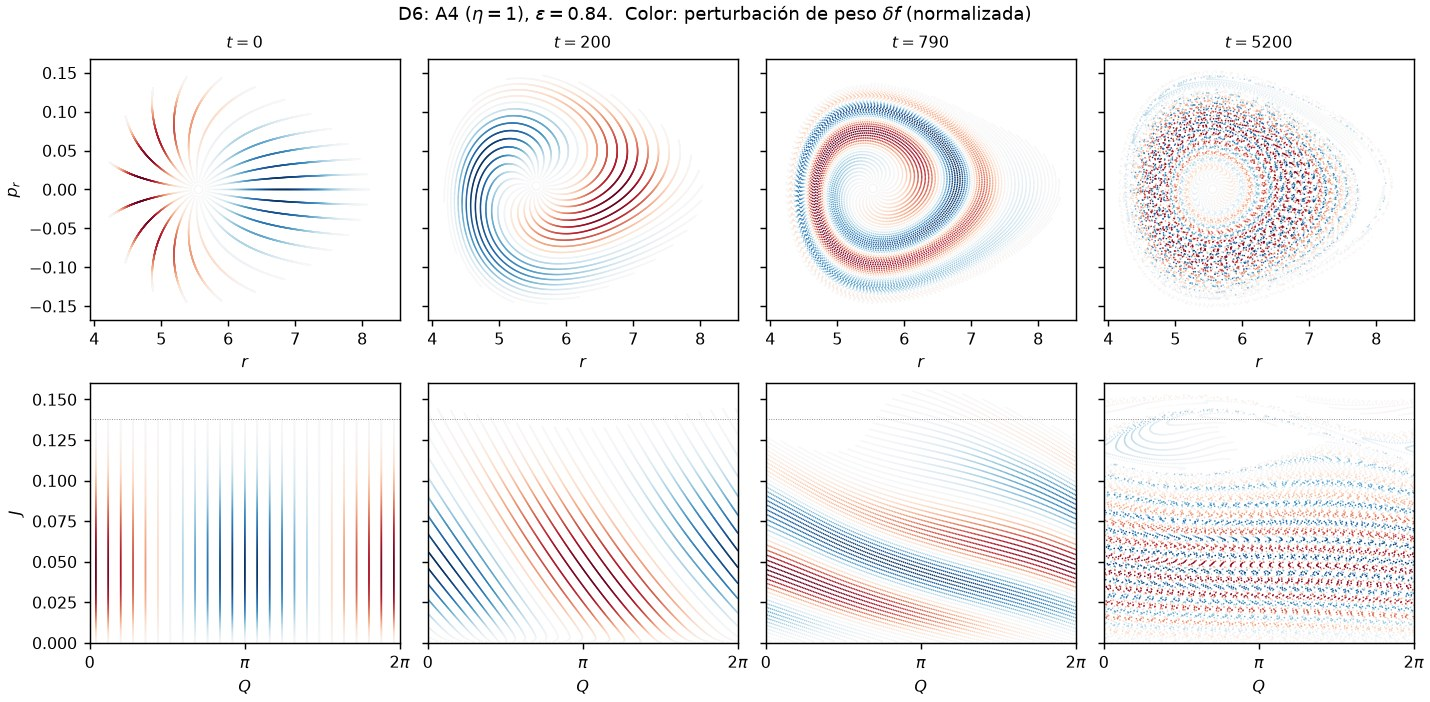
\includegraphics[width=\textwidth]{fase_D6.jpg}
\caption{D6: $\eta=1$, $\varepsilon=0.84$. Al final ($t=5200$) las filas con $J\gtrsim0.11$ se
enrollan alrededor de un punto: la isla de partículas atrapadas por la onda,
junto a la resonancia $\Omega(J)=\omega$ cerca del borde. El cambio de acción llega a
$0.048$.}
\label{fig:fase_D6}
\end{figure}

\begin{figure}[p]
\centering
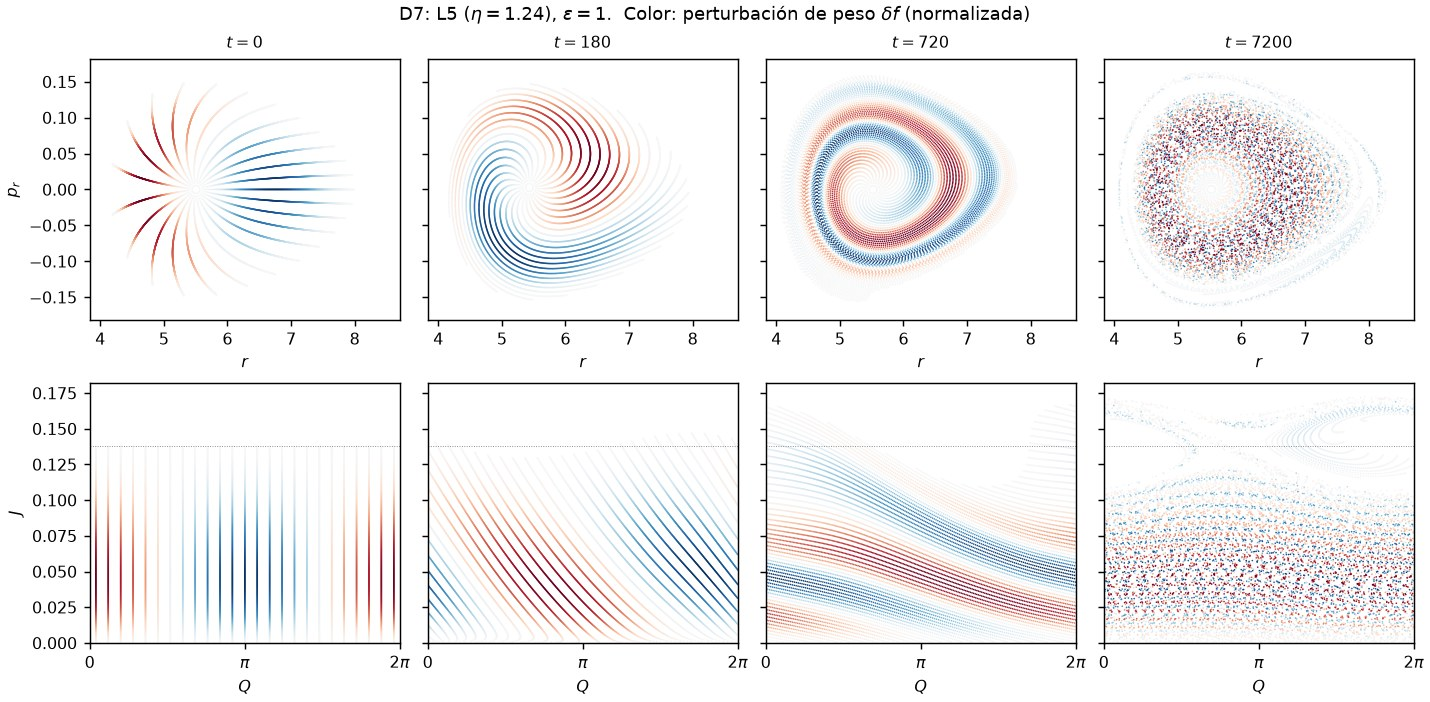
\includegraphics[width=\textwidth]{fase_D7.jpg}
\caption{D7: $\eta=1.24$, $\varepsilon=1$. Ya en $t=720$ las filas se ondulan, y al final
hay una isla junto al borde, con partículas hasta $J=0.179$, fuera del soporte.
El cambio de acción llega a $0.073$, más de la mitad del soporte.}
\label{fig:fase_D7}
\vspace{1.5em}
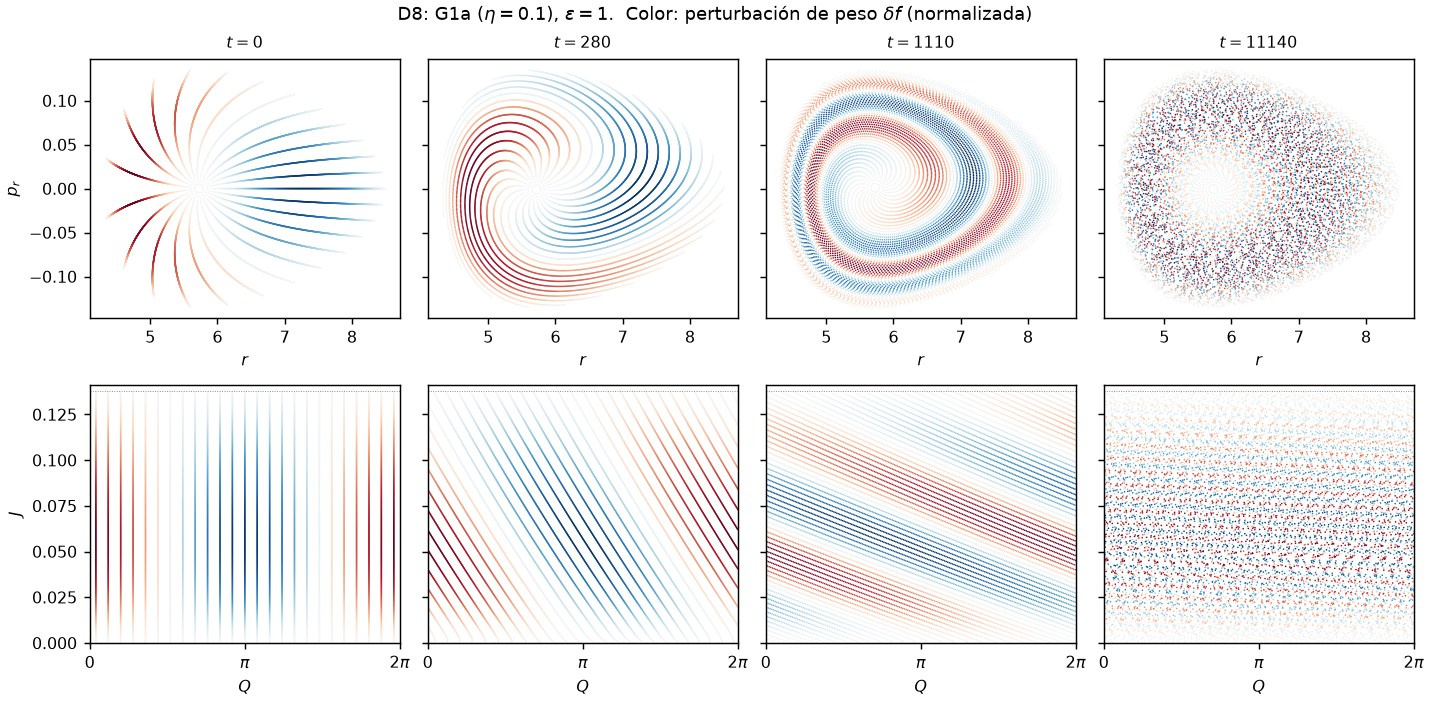
\includegraphics[width=\textwidth]{fase_D8.jpg}
\caption{D8: $\eta=0.1$, $\varepsilon=1$, borde abrupto ($g=1$). Como D1: en espacio fase
la diferencia entre los bordes no se ve, porque la respuesta que persiste en el
borde es de $10^{-3}$ del valor inicial.}
\label{fig:fase_D8}
\end{figure}

\section{Los videos}
\label{sec:videos}

Hay un video por simulación, catorce en total, en
\texttt{reproducir/\allowbreak videos/\allowbreak demo\_\allowbreak eta/\allowbreak <corrida>.mp4} (fuera del control de
versiones; se regeneran con \texttt{demo\_eta.py videos}). Tienen 1280$\times$720
píxeles, un cuadro por instantánea (cada 10 unidades de tiempo, unas ocho por
vuelta radial) y 30 cuadros por segundo: de 15 s (D2) a 57 s (D5 y Z\_A4). Cada
cuadro tiene cuatro paneles:
\begin{itemize}
\item arriba a la izquierda, las partículas en $(r,p_r)$, coloreadas por su
perturbación de peso como en la sección~\ref{sec:fase}: ahí se ve la mezcla;
\item arriba a la derecha, en $(Q,J)$, coloreadas por su acción \emph{inicial}, como
en la figura~\ref{fig:islas}: ahí se ve el cambio de acción. En la mezcla libre
cada color se queda en su fila; una fila que se deforma, o que cruza el borde
$J_t$ (línea punteada), cambió de acción por el campo propio;
\item abajo a la izquierda, el perfil $\delta\Phi_\varepsilon(r)$ de la PIC y el de la teoría
lineal en ese instante, con el eje vertical reescalado a la envolvente para que
el perfil se siga viendo mientras decae;
\item abajo a la derecha, la envolvente de $\|\delta\Phi\|$ en todo el tiempo, PIC y
lineal, con una línea que marca el instante del cuadro.
\end{itemize}
En los videos de las corridas Z el color en $(r,p_r)$ es la etiqueta $\cos Q_0$, y
los paneles de abajo muestran el $\delta\Phi$ propio de la corrida sin perturbación,
relativo al potencial del equilibrio: la parte estática es el error de
discretización del equilibrio, y la oscilación, su piso de ruido.

\paragraph{Qué mirar.} En D1 y D2, cómo la espiral se aprieta mientras el perfil
de $\delta\Phi$ se apaga. En D3 y D4, que el perfil sigue oscilando igual a los
$20\,\tau_1$ aunque las partículas ya se mezclaron: el modo es colectivo, no un grupo
de partículas. En D6 y D7, la formación de la isla en $(Q,J)$. En D5, el final:
la curva de la PIC se despega de la lineal y deja de bajar.

\section{Lo que sigue}
\label{sec:siguiente}

La demo muestra que las tres preguntas del estudio $\eta$ tienen respuesta
medible con el código. Para convertir estas observaciones en resultados:
\begin{enumerate}
\item \textbf{Convergencia de lo que la teoría lineal no predice.} La pérdida de
D3, la amplitud tardía de D5 y el enrollamiento de D6 no deben cambiar al partir
$\Delta t$ a la mitad y al cuadruplicar $N$ (bloque~B de la batería). Con $N$ mayor se
sabrá también si la estructura fina de D5 es ruido: si lo es, baja como
$N^{-1/2}$.
\item \textbf{El criterio para los modos discretos.} Un barrido en $\varepsilon$ de D3,
de $0.1$ a $0.003$, debe mostrar que la pérdida desaparece cuando
$\omega_b<\Omega_{\min}-\omega$.
\item \textbf{El mapa $(\eta,\nu)$ completo} del lado amortiguado, con corridas más
largas en D5 y D6 para ver si la amplitud oscila con el periodo de rebote y dónde
se satura.
\item \textbf{El borde abrupto a tiempos largos}, con $\varepsilon\approx0.3$--$0.5$, la
amplitud que minimiza el piso, y restando la parte estática, para seguir la
respuesta de D8 más allá de $15\,\tau_1$.
\end{enumerate}
El diseño completo, con 30 corridas y su costo, está en la batería $\eta$.

\appendix

\section{Las corridas de referencia}
\label{sec:ref}

Las seis corridas Z tienen el mismo equilibrio y las mismas posiciones iniciales
que sus corridas D, sin perturbación. El color es solo la etiqueta $\cos Q_0$: el
patrón se enrolla igual que en las D porque las partículas giran con sus
frecuencias, pero la densidad no cambia, y las filas de $J$ quedan horizontales:
el cambio máximo de acción es menor que $10^{-3}$. Es la comprobación visual de
que el equilibrio discreto es estacionario.

\begin{figure}[p]
\centering
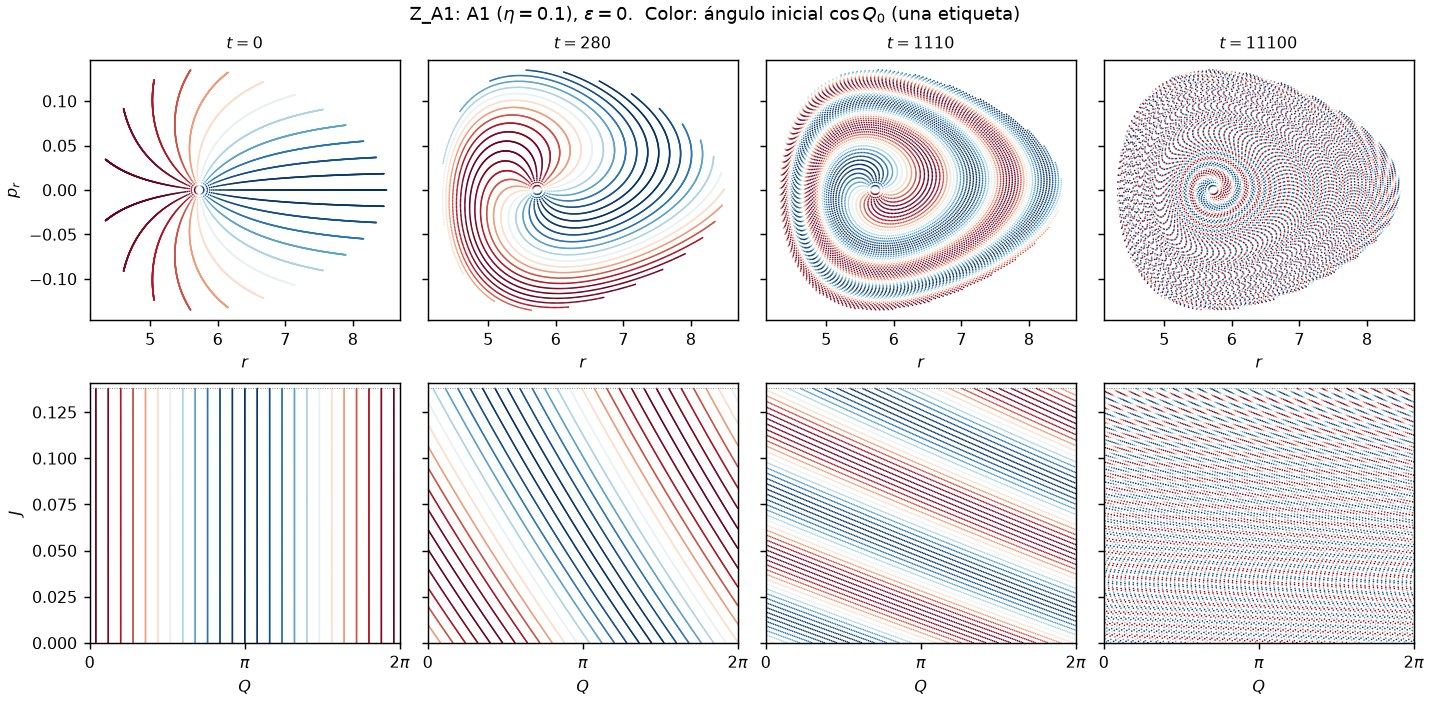
\includegraphics[width=0.92\textwidth]{fase_Z_A1.jpg}\\[0.8em]
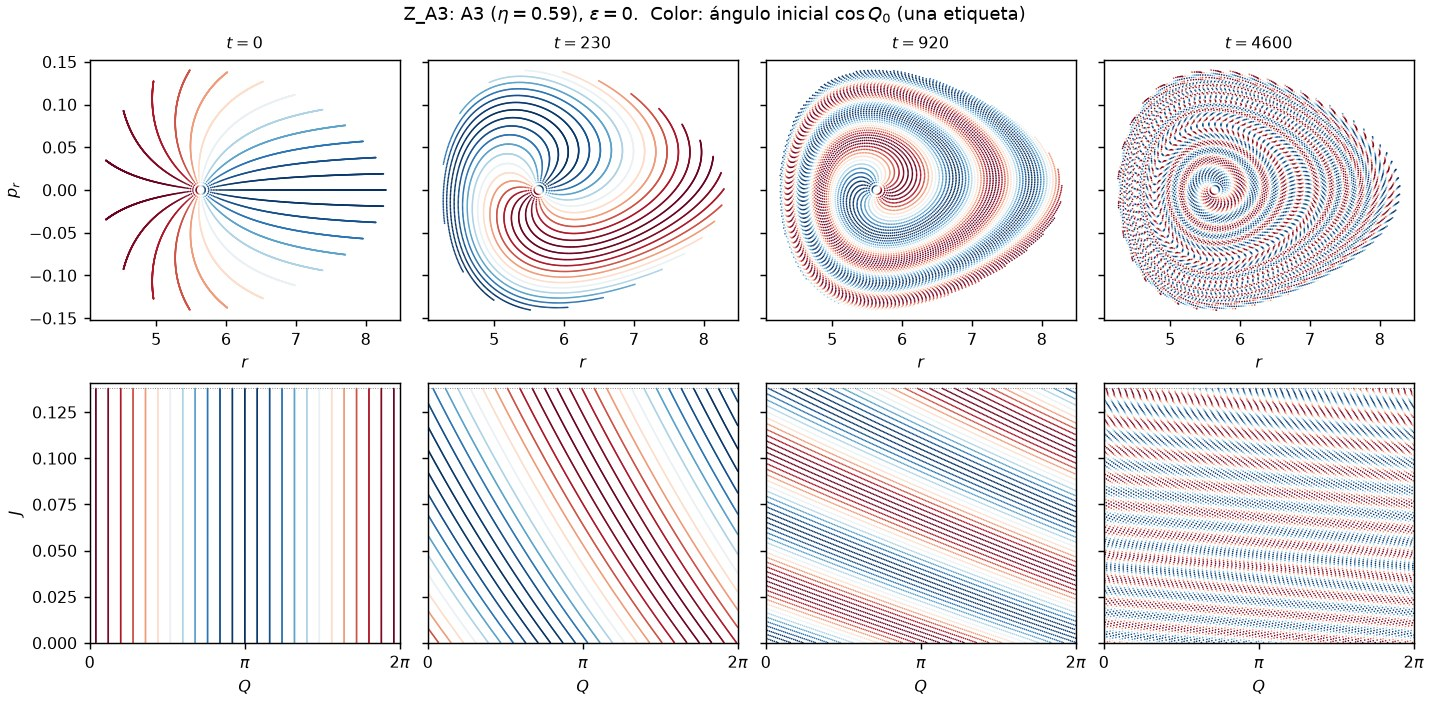
\includegraphics[width=0.92\textwidth]{fase_Z_A3.jpg}\\[0.8em]
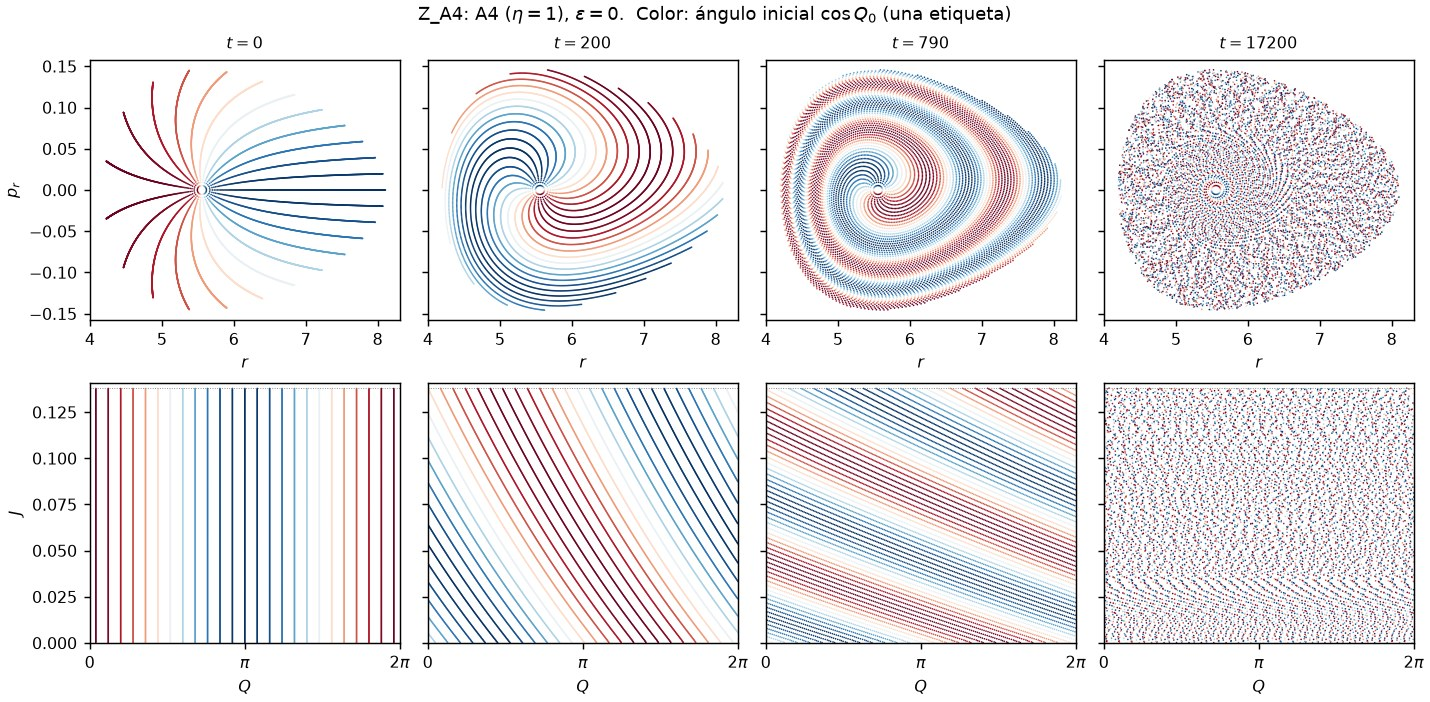
\includegraphics[width=0.92\textwidth]{fase_Z_A4.jpg}
\caption{Referencias de A1 (D1), A3 (D2) y A4 (D5 y D6).}
\label{fig:fase_Z1}
\end{figure}

\begin{figure}[p]
\centering
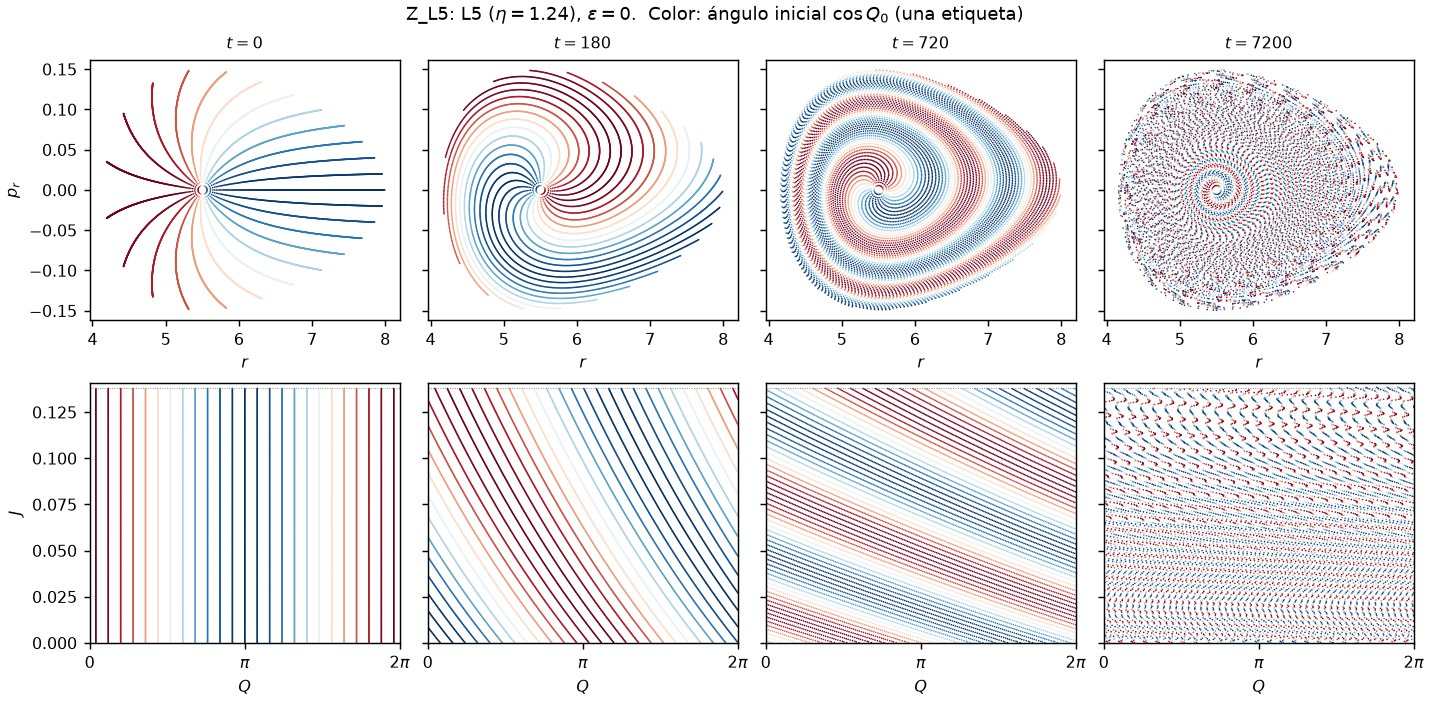
\includegraphics[width=0.92\textwidth]{fase_Z_L5.jpg}\\[0.8em]
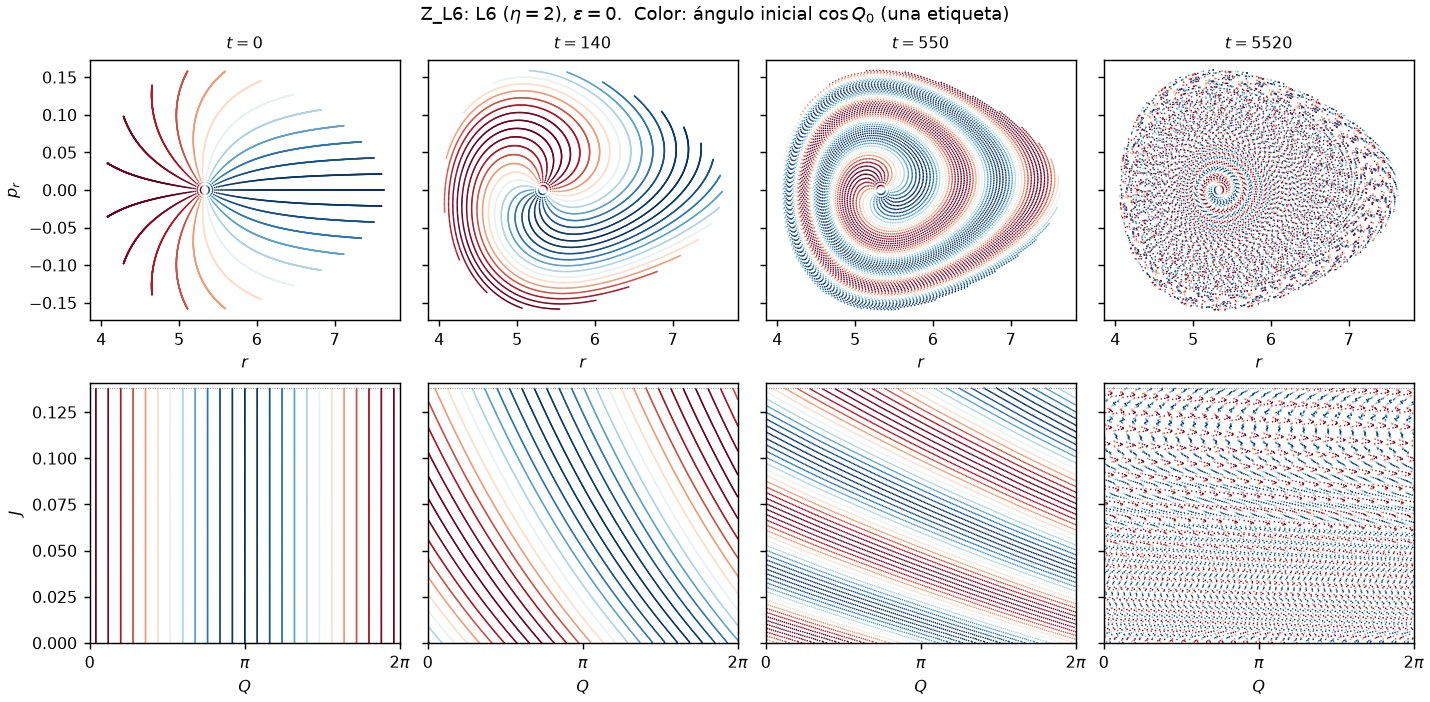
\includegraphics[width=0.92\textwidth]{fase_Z_L6.jpg}\\[0.8em]
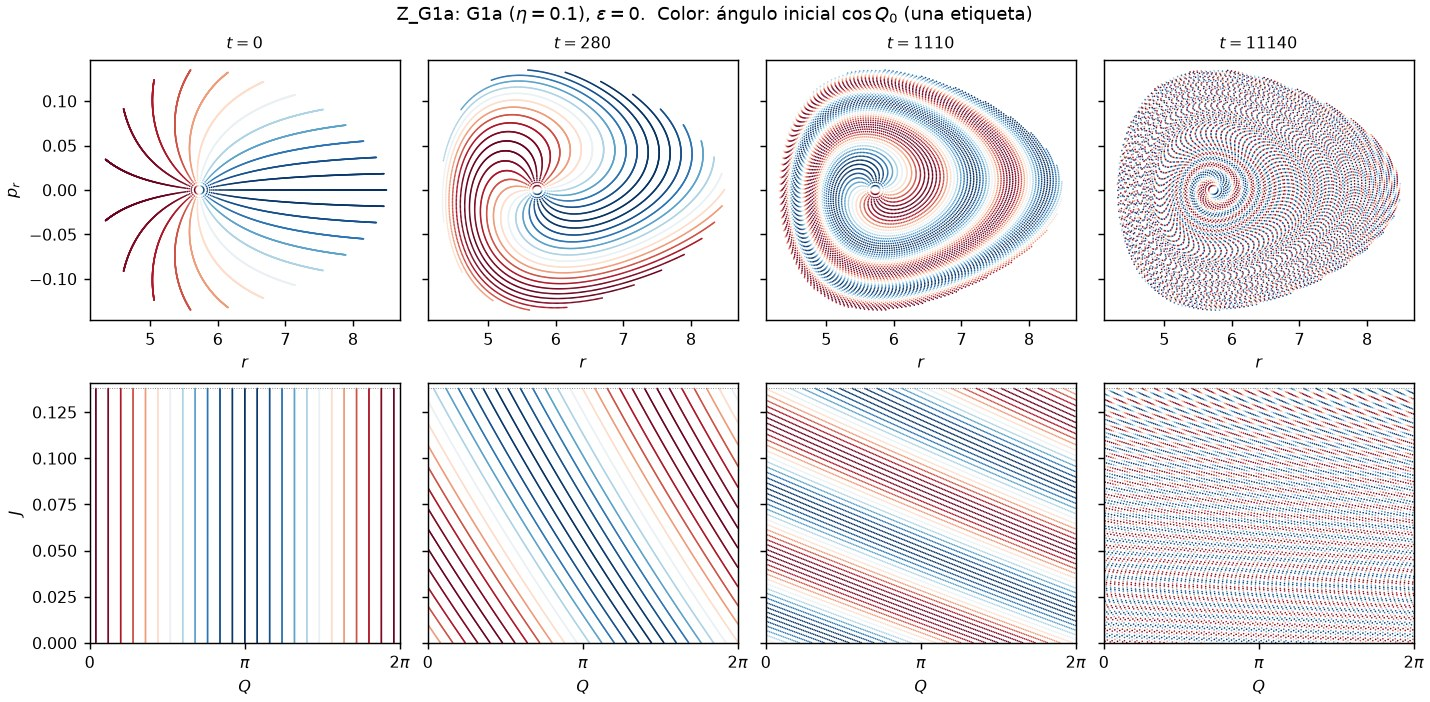
\includegraphics[width=0.92\textwidth]{fase_Z_G1a.jpg}
\caption{Referencias de L5 (D3 y D7), L6 (D4) y G1a (D8).}
\label{fig:fase_Z2}
\end{figure}

\section{Cómo reproducir la demo}
\label{sec:reproducir}

Todo el flujo está en \texttt{reproducir/scripts/demo\_eta.py}, en seis pasos que
se corren desde ese directorio y reutilizan lo que ya exista:
\begin{center}
\small
\begin{tabular}{lL{9.6cm}r}
\toprule
paso & qué hace & tiempo\\
\midrule
\texttt{preparar} & 14 estados iniciales con \texttt{equilibrio.py} y sus \texttt{.par} en \texttt{reproducir/corridas/12\_demo\_eta/} & \SI{4}{min}\\
\texttt{lineal} & las 6 soluciones lineales con \texttt{lineal.py}, hasta el $t_{\rm fin}$ más largo de cada equilibrio & \SI{13}{min}\\
\texttt{correr} & las 14 corridas PIC, una tras otra, con 4 hilos & \SI{3}{h}\\
\texttt{analizar} & mapa ángulo-acción de cada instantánea (una sola vez), $h_k$, $\delta\Phi$; 4 procesos & \SI{55}{min}\\
\texttt{figuras} & espacio fase, series y \texttt{exe/demo\_eta/resumen.txt} & \SI{2}{min}\\
\texttt{videos} & un video por corrida, 4 a la vez & \SI{50}{min}\\
\bottomrule
\end{tabular}
\end{center}
Las salidas ocupan \SI{2.6}{GB} en \texttt{exe/demo\_eta/}, fuera del control de
versiones.





\end{document}
